\section{问题描述}

本题研究某海域鲨鱼（捕食者）与金枪鱼（猎物）种群数量的动态变化。已知二者满足Lotka-Volterra捕食者-猎物模型，模型的微分方程组如下：

\[
\begin{cases}
\dfrac{dS}{dt} = a_1 S T - a_2 S \\[1em]
\dfrac{dT}{dt} = a_3 T - a_4 S T
\end{cases}
\]

其中 $S(t)$ 表示鲨鱼数量，$T(t)$ 表示金枪鱼数量。参数取值：
\[
a_1 = 0.015,\quad a_2 = 0.7,\quad a_3 = 0.5,\quad a_4 = 0.01.
\]
初始条件：
\[
S(0) = 100,\quad T(0) = 100.
\]

题目要求采用显式Euler法和四阶Runge-Kutta法（可以使用ode45直接求解，也可以自编代码）以及Simulink软件，求解未来100年内两种群数量的变化，时间步长取 $\Delta t = 0.001$ 年（有余力的可以尝试取 $\Delta t = 0.1$ 年），并对比分析结果。



\section{数值方法原理}

\subsection{显式Euler法}

Euler法是一阶显式单步法，格式为：
\[
\mathbf{y}_{n+1} = \mathbf{y}_n + \Delta t \cdot \mathbf{f}(t_n, \mathbf{y}_n).
\]
对于本模型，每一步更新：
\[
\begin{aligned}
S_{n+1} &= S_n + \Delta t (a_1 S_n T_n - a_2 S_n), \\
T_{n+1} &= T_n + \Delta t (a_3 T_n - a_4 S_n T_n).
\end{aligned}
\]

\subsection{四阶Runge-Kutta法（RK4）}

四阶Runge-Kutta法具有四阶的精度（画外音：怎么总感觉这句话怪怪的）。这一方法每步计算四个斜率：
\[
\begin{aligned}
\mathbf{k}_1 &= \mathbf{f}(t_n, \mathbf{y}_n), \\
\mathbf{k}_2 &= \mathbf{f}(t_n + \tfrac{\Delta t}{2}, \mathbf{y}_n + \tfrac{\Delta t}{2}\mathbf{k}_1), \\
\mathbf{k}_3 &= \mathbf{f}(t_n + \tfrac{\Delta t}{2}, \mathbf{y}_n + \tfrac{\Delta t}{2}\mathbf{k}_2), \\
\mathbf{k}_4 &= \mathbf{f}(t_n + \Delta t, \mathbf{y}_n + \Delta t \mathbf{k}_3), \\
\mathbf{y}_{n+1} &= \mathbf{y}_n + \frac{\Delta t}{6}(\mathbf{k}_1 + 2\mathbf{k}_2 + 2\mathbf{k}_3 + \mathbf{k}_4).
\end{aligned}
\]

将 $\mathbf{y} = [S, T]^\mathrm{T}$ 和右端函数代入即可。


\section{MATLAB运行结果及分析}

使用自编的Euler法和RK4法程序以及MATLAB自带的ode45方法，分别取步长 $\Delta t = 0.001$ 和 $\Delta t = 0.1$，计算时间区间 $[0,100]$ 年的种群数量。以下是实验的结果，采用图片进行展示。

\subsection{步长 $\Delta t = 0.001$ 年}
在步长 $\Delta t = 0.001$ 年时，三种方法得到的结果如下，这里直接画图展示：
\begin{figure}[h]
    \centering
    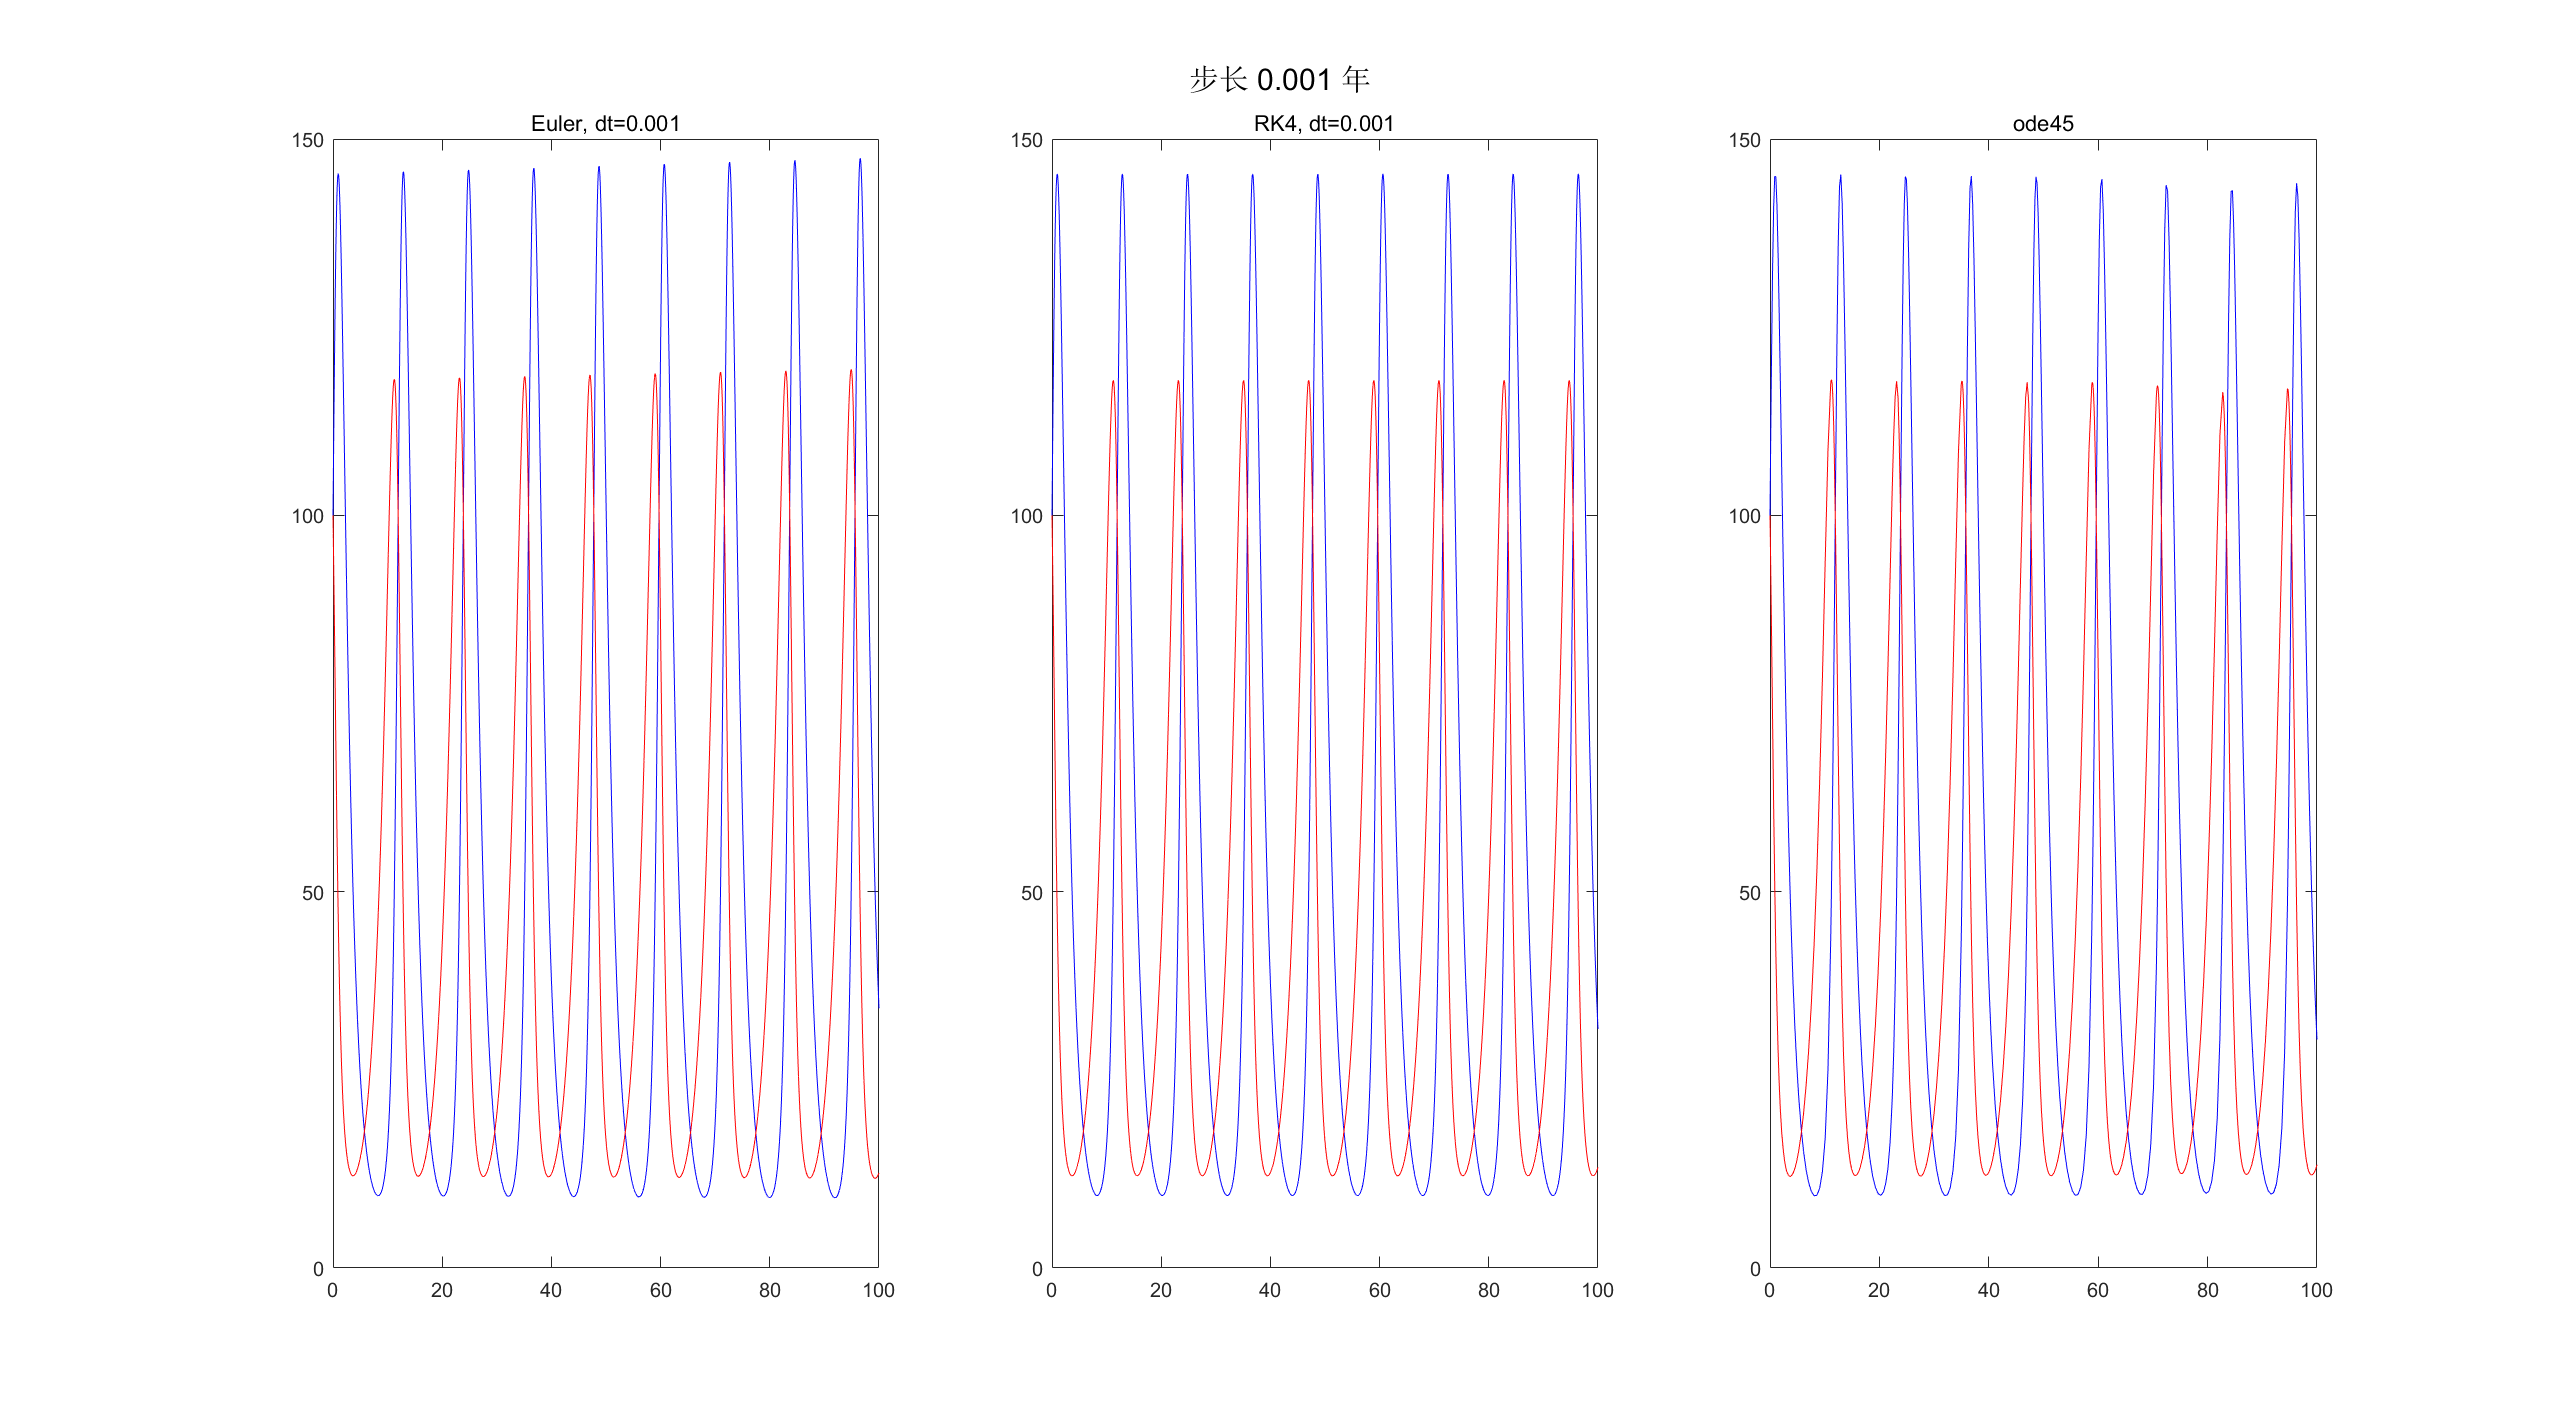
\includegraphics[width=0.75\linewidth]{figure/HW1/dt0.001.png}
    \caption{dt=0.001时的三种方法}
\end{figure}

此时，三种方法均得到稳定的周期振荡，周期约为20年。鲨鱼和金枪鱼数量交替达到峰值，且振幅基本保持不变。由于步长足够小，Euler法与RK4法结果几乎重合，说明此时Euler法也能获得良好精度。

\subsection{步长 $\Delta t = 0.1$ 年}
在步长 $\Delta t = 0.1$ 年时，三种方法得到的结果如下，这里依旧直接画图展示：
\begin{figure}[h]
    \centering
    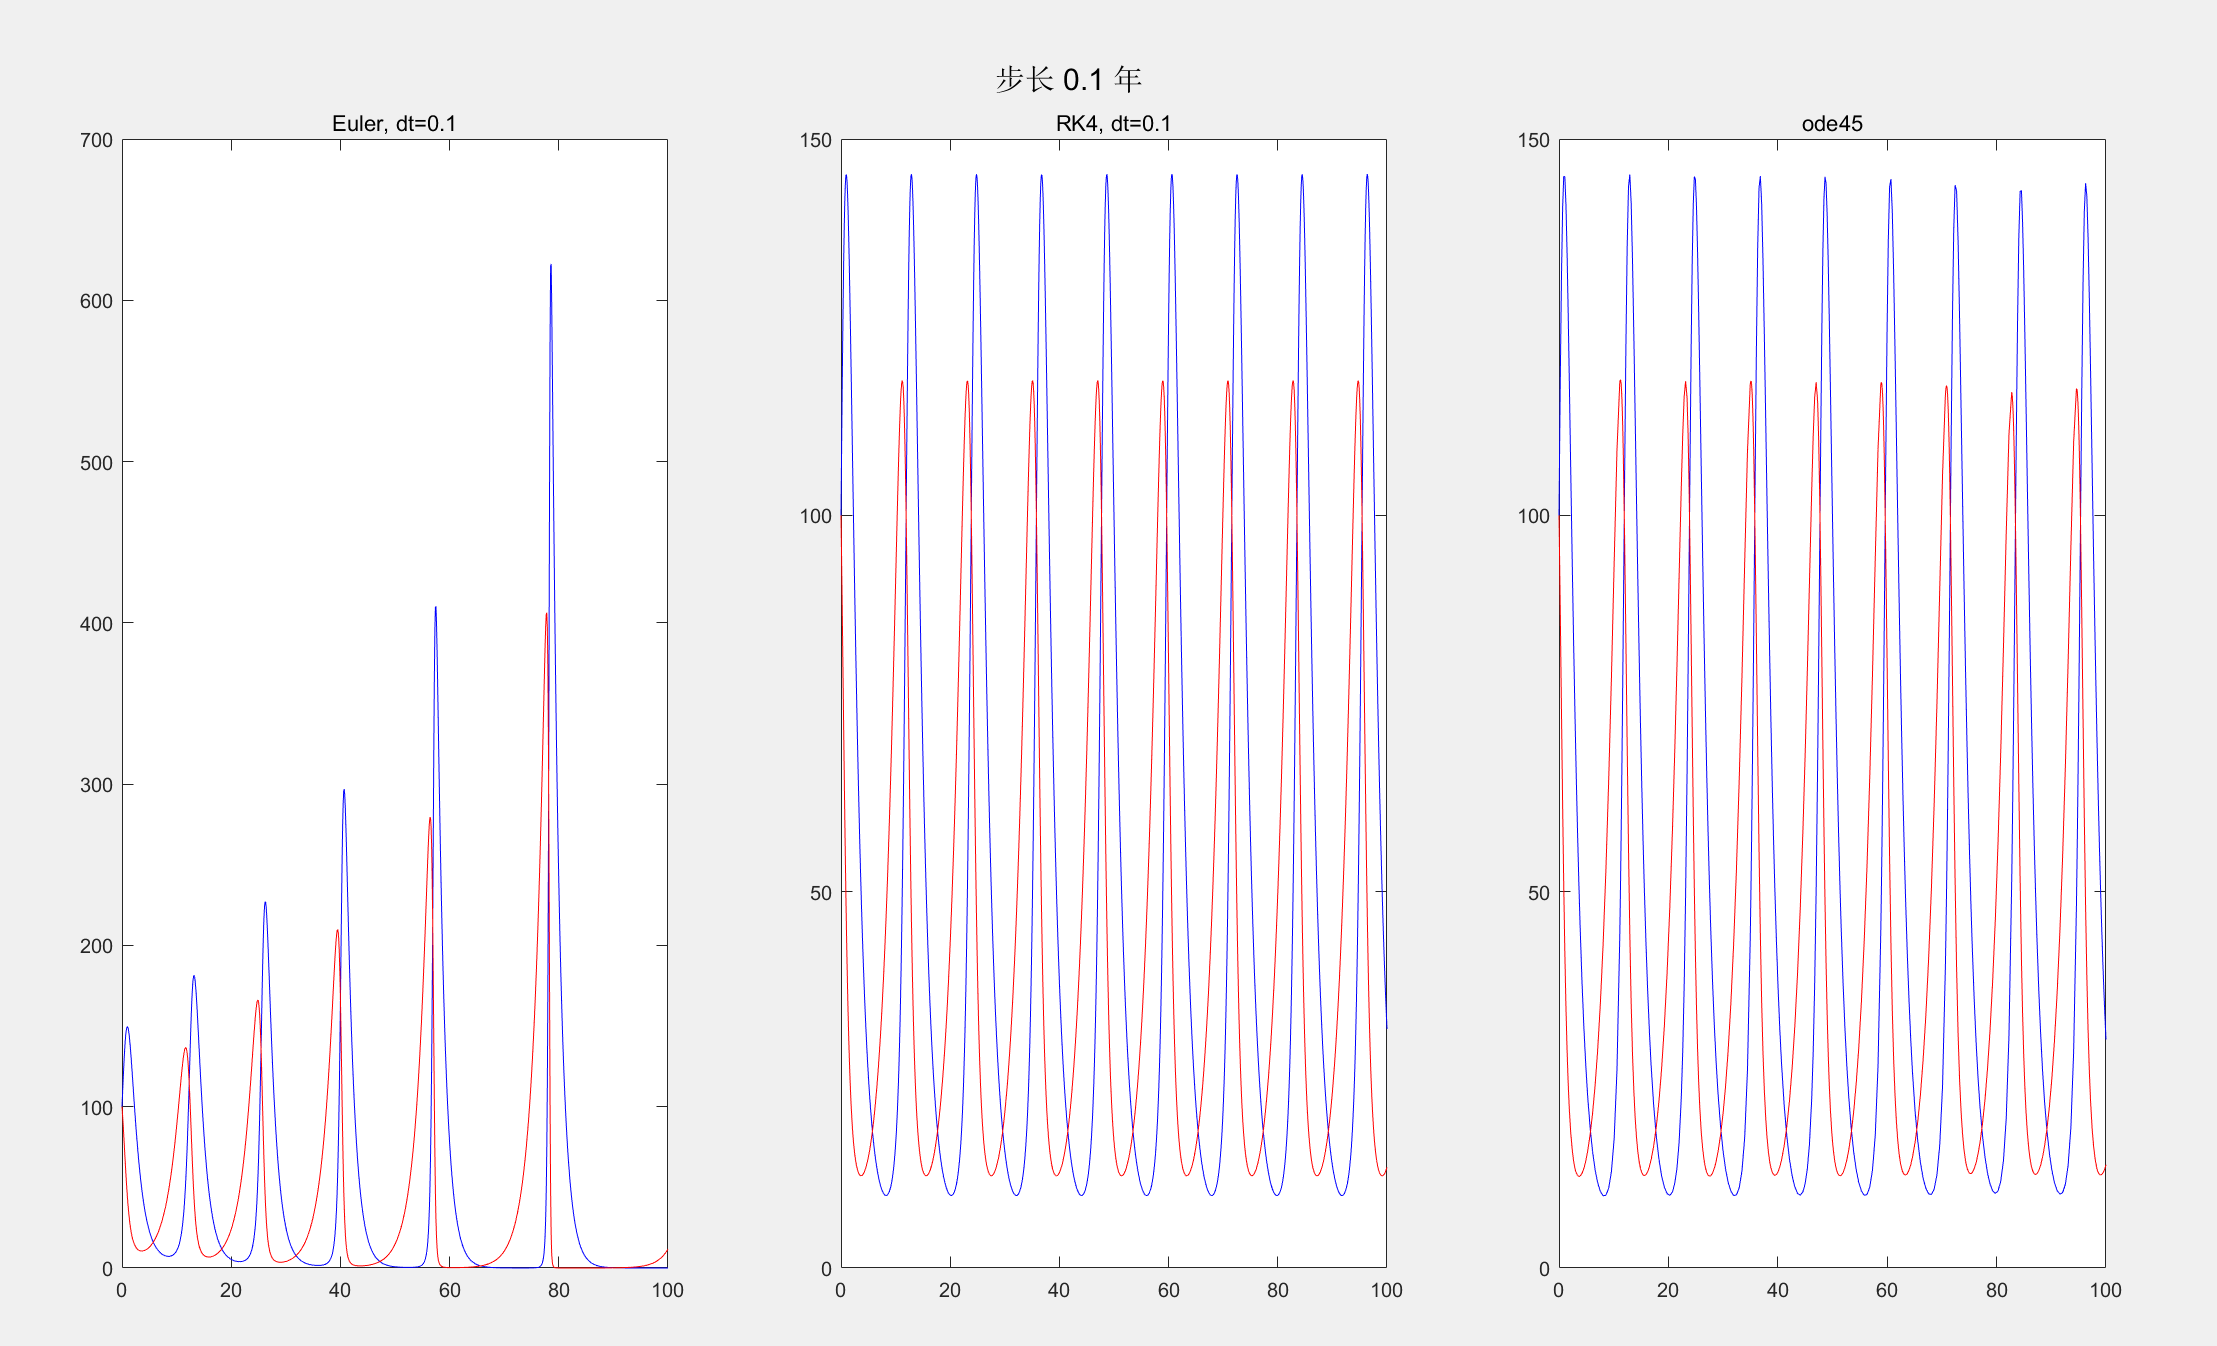
\includegraphics[width=0.75\linewidth]{figure/HW1/dt0.1.png}
    \caption{dt=0.1时的三种方法}
\end{figure}
不难注意到，这里Euler法步长 $\Delta t = 0.001$ 年时的情况出现了差异。接下来单独分析一下两种方法的差异性。
\begin{itemize}
    \item \textbf{Euler 法}：数值仿真曲线在计算初期仍能够维持正常的振荡变化规律，但随着仿真时间不断推进，波形振幅出现持续非理性增大的现象，计算结果逐步偏离真实物理规律。该现象本质源于显式 Euler 法本身严苛的稳定性约束，当仿真时间步长选取过大时，格式稳定性条件无法满足，直接造成算法失效、计算精度彻底失控。
    \item \textbf{四阶Runge-Kutta法}：在相同放大时间步长的测试条件下，整体仿真曲线依旧保持光滑连续，振荡形态稳定可靠，计算结果与高精度小步长 $\Delta t=0.001$ 工况下的基准曲线高度吻合。这一对比结果充分验证了 RK4 算法具备更优异的长期数值稳定性与容错能力，对计算步长的宽容度更高。这说明工程仿真中可在保证精度前提下选用更大步长以提升整体计算效率。
\end{itemize}


\subsection{Simulink仿真结果}

在Simulink中搭建模型，分别选择ode4（RK4）和ode1（Euler）作为求解器，同时采用固定步长方法，步长分别设为$\Delta t = 0.001$ 和 $\Delta t = 0.1$。
搭建的结果如示例图：
\begin{figure}[H]
    \centering
    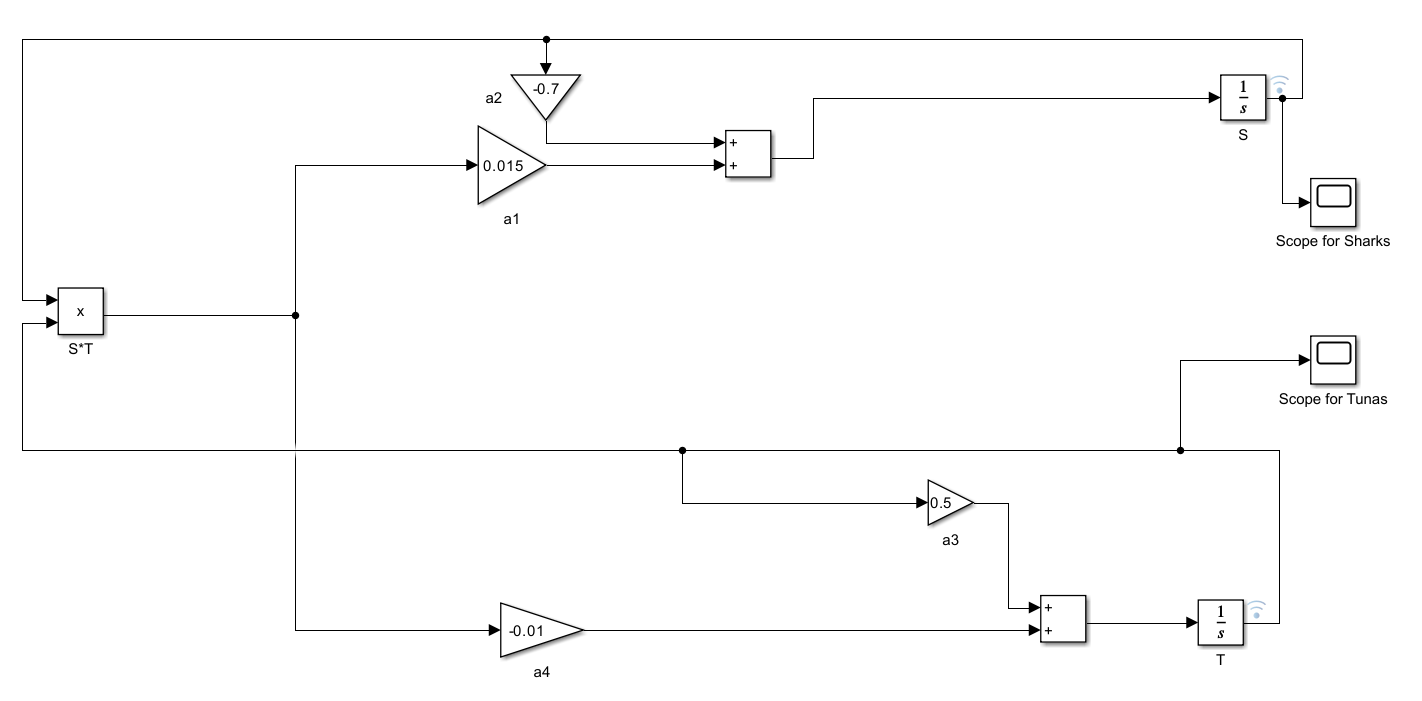
\includegraphics[width=0.75\linewidth]{figure/HW1/simulink.png}
    \caption{Simulink建模示例图}
\end{figure}
.slx文件详见支持文档的code附录。
\par
仿真结果如下图所示。
\begin{figure}[h]
    \centering
    \begin{minipage}{0.48\textwidth}
        \centering
        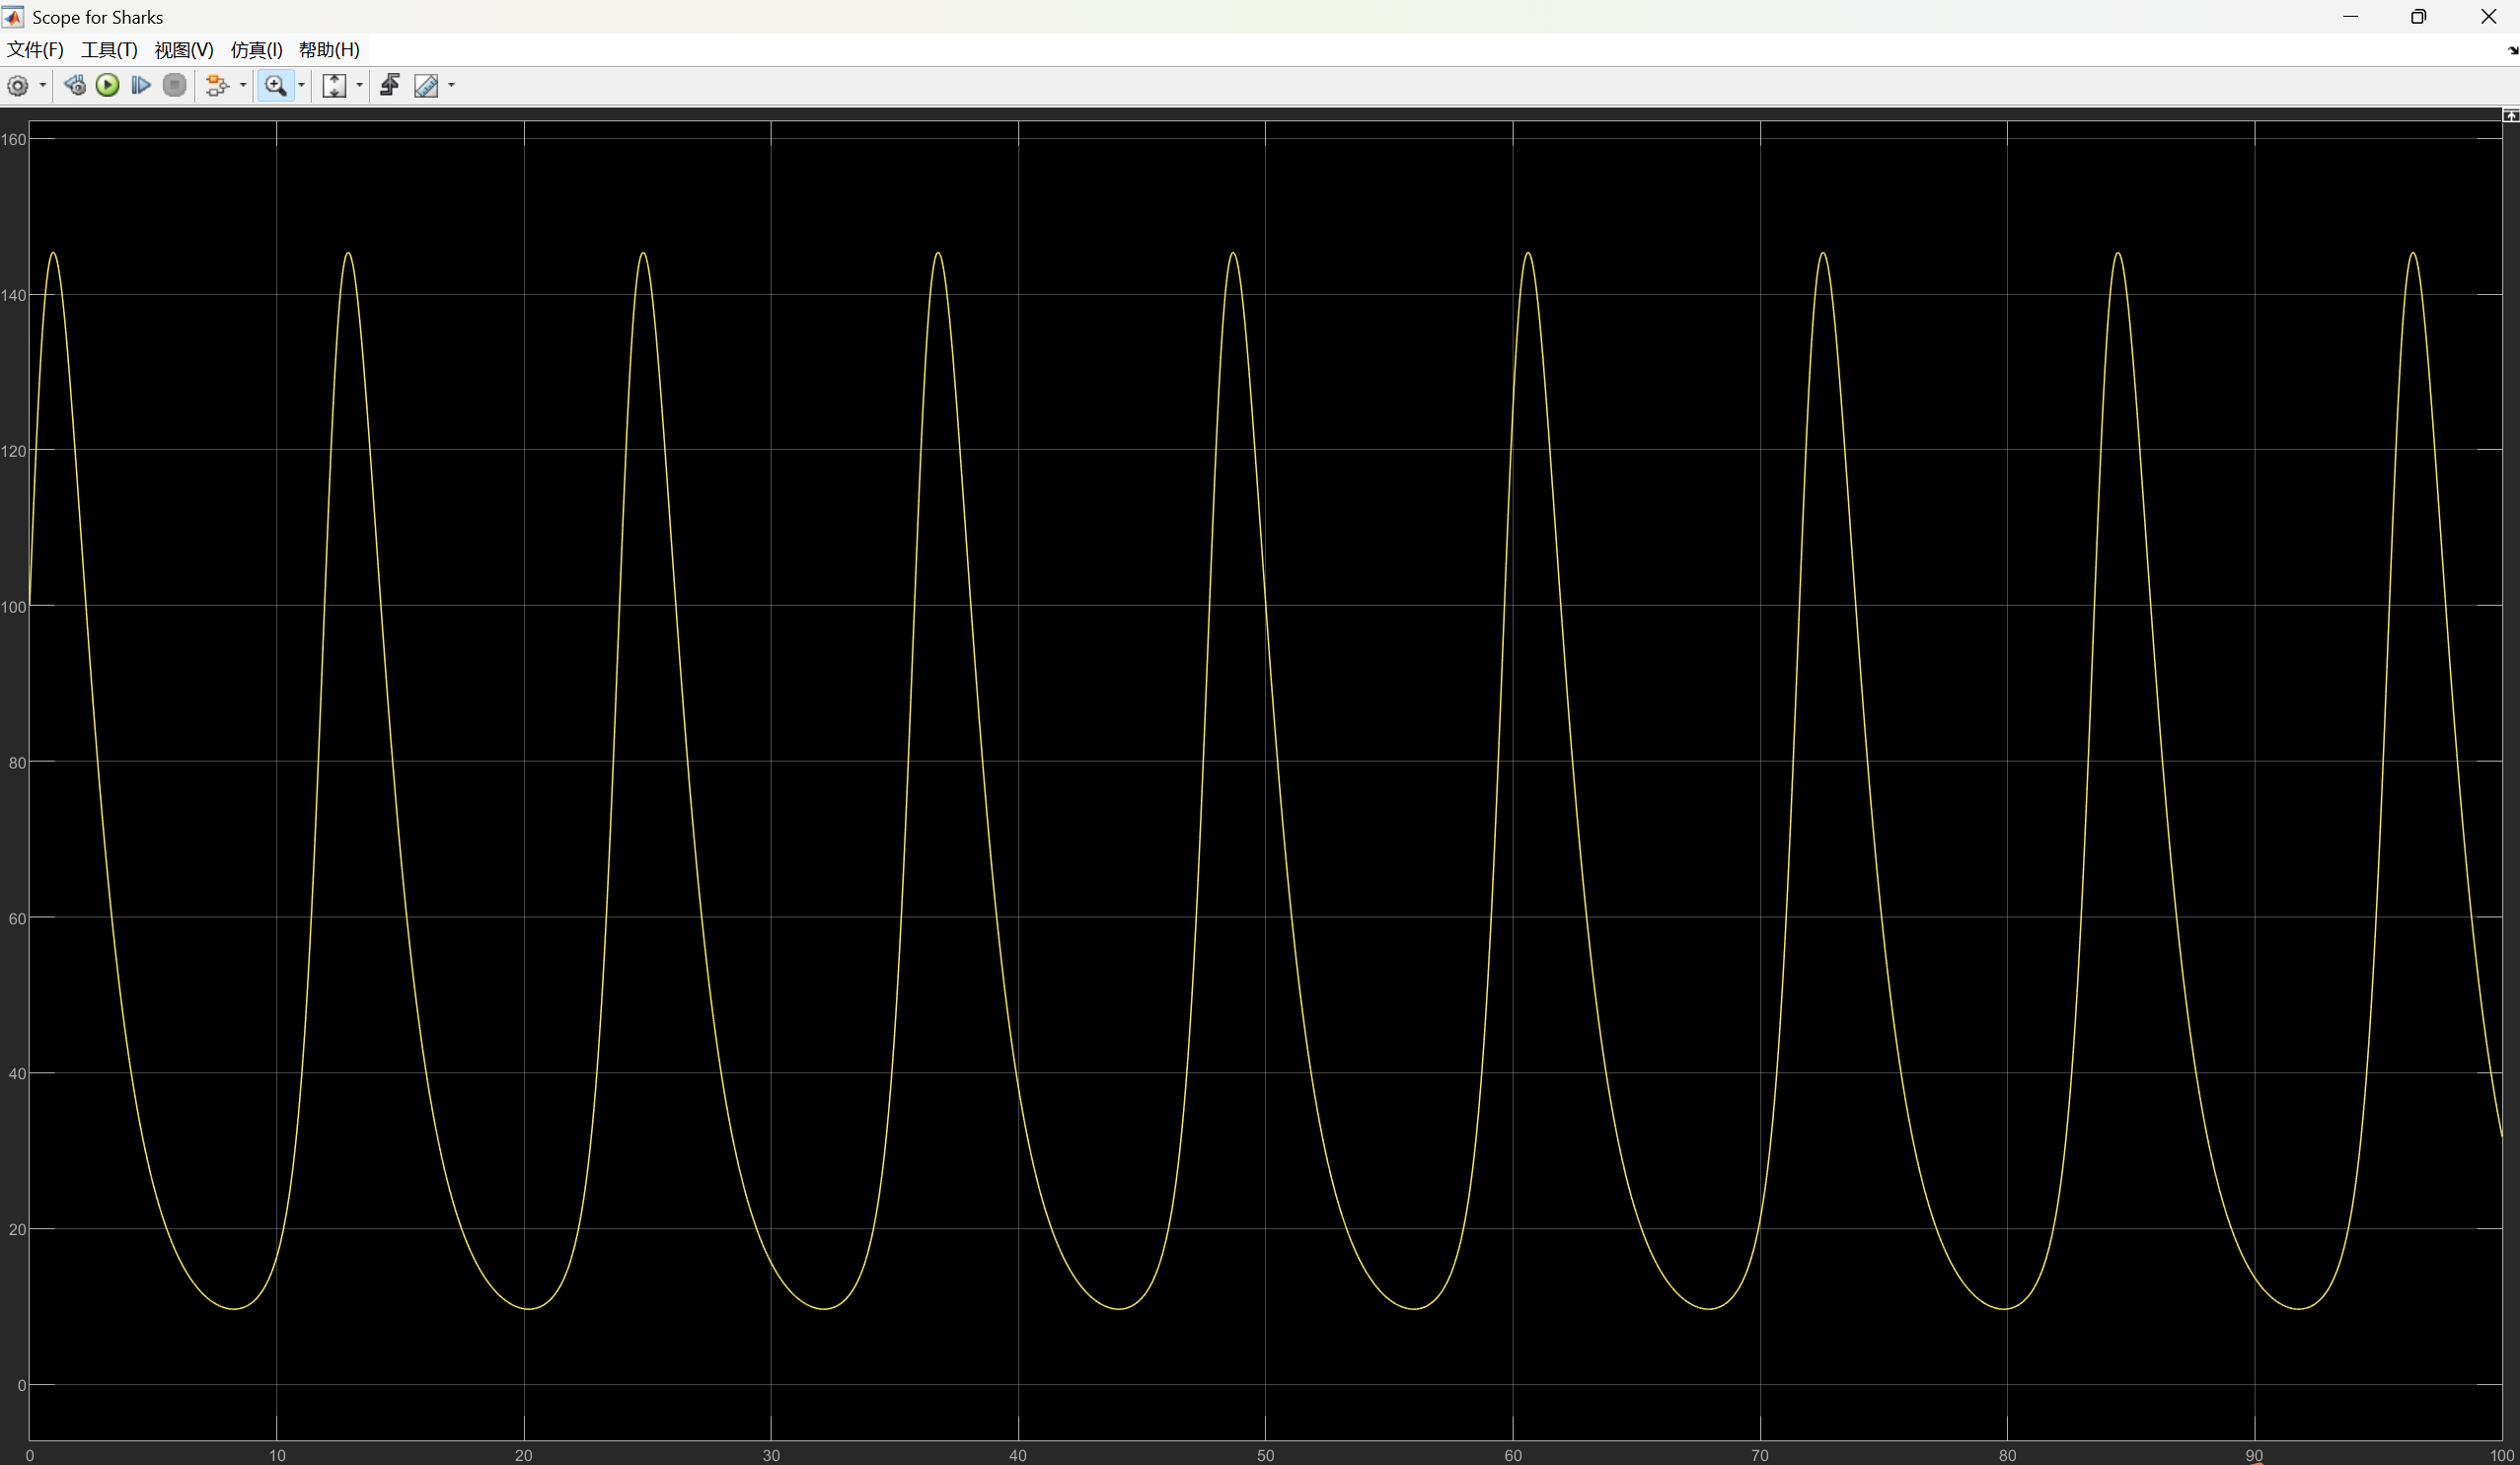
\includegraphics[width=\linewidth]{figure/HW1/ode4S0.001.png}
    \end{minipage}
    \hfill
    \begin{minipage}{0.48\textwidth}
        \centering
        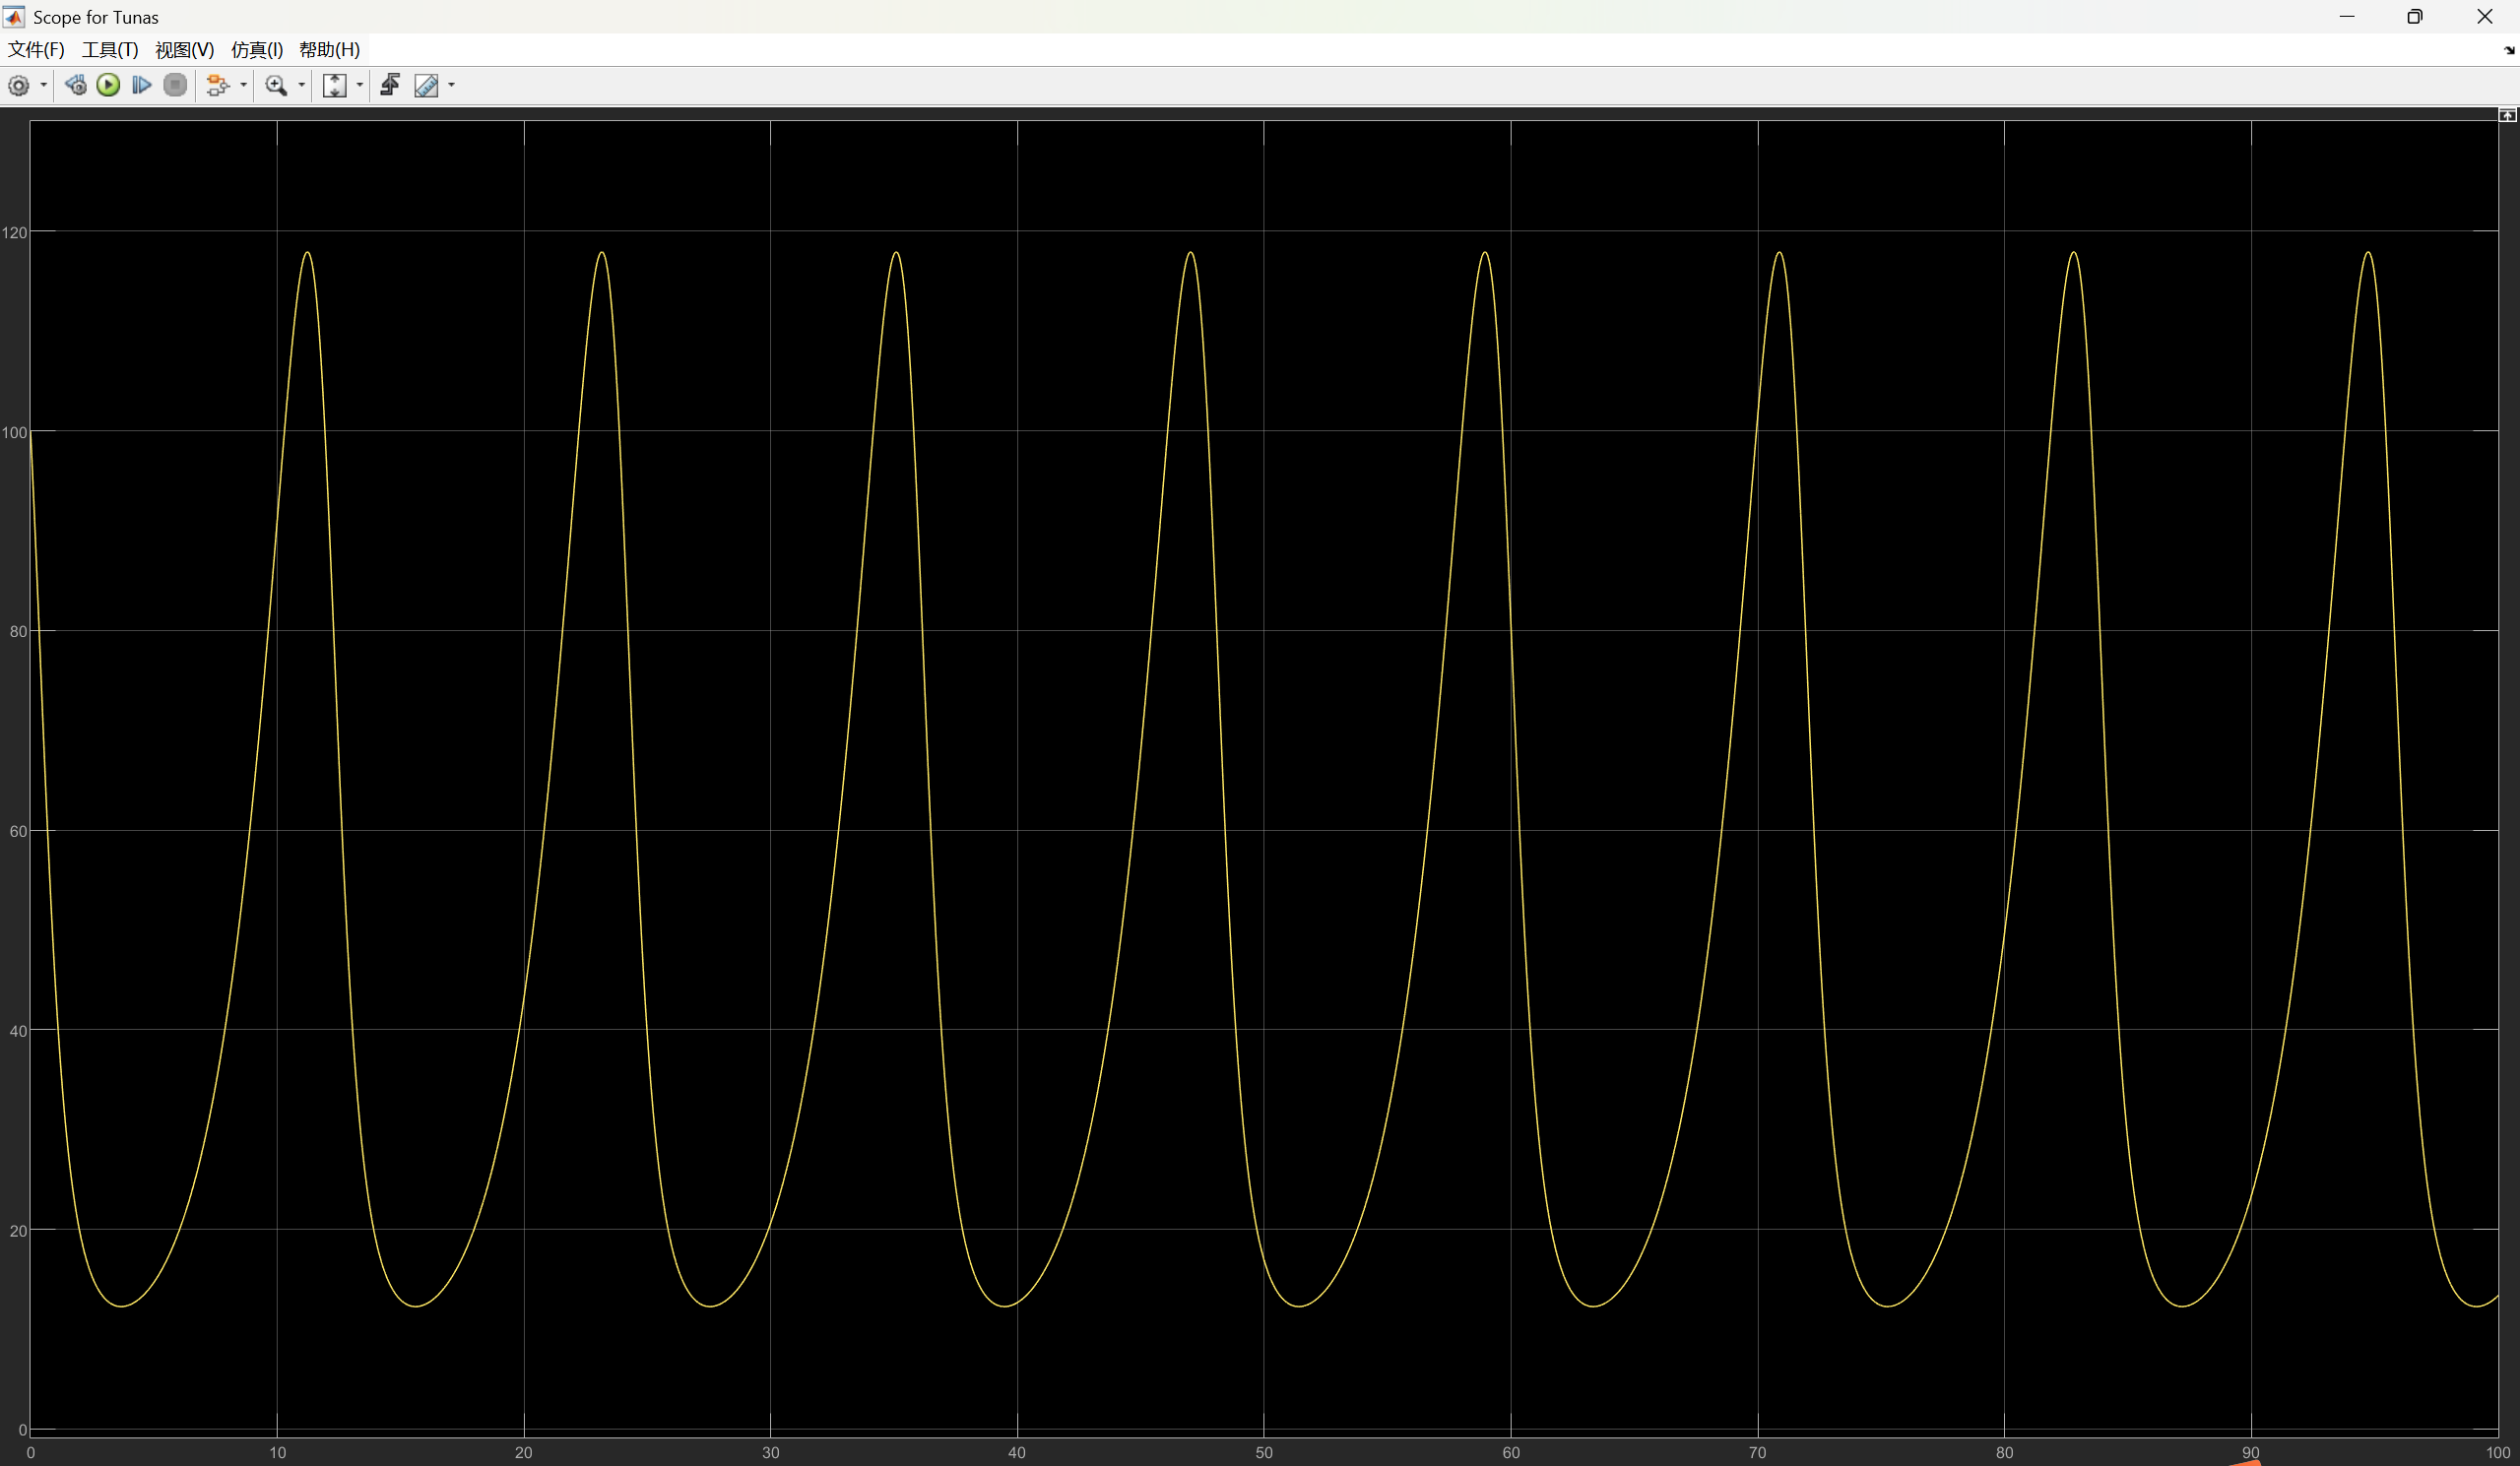
\includegraphics[width=\linewidth]{figure/HW1/ode4T0.001.png}
    \end{minipage}
    \caption{$\Delta t=0.001$ 时 ode4S 与 ode4T 数值结果}
\end{figure}
\begin{figure}[h]
    \centering
    \begin{minipage}{0.48\textwidth}
        \centering
        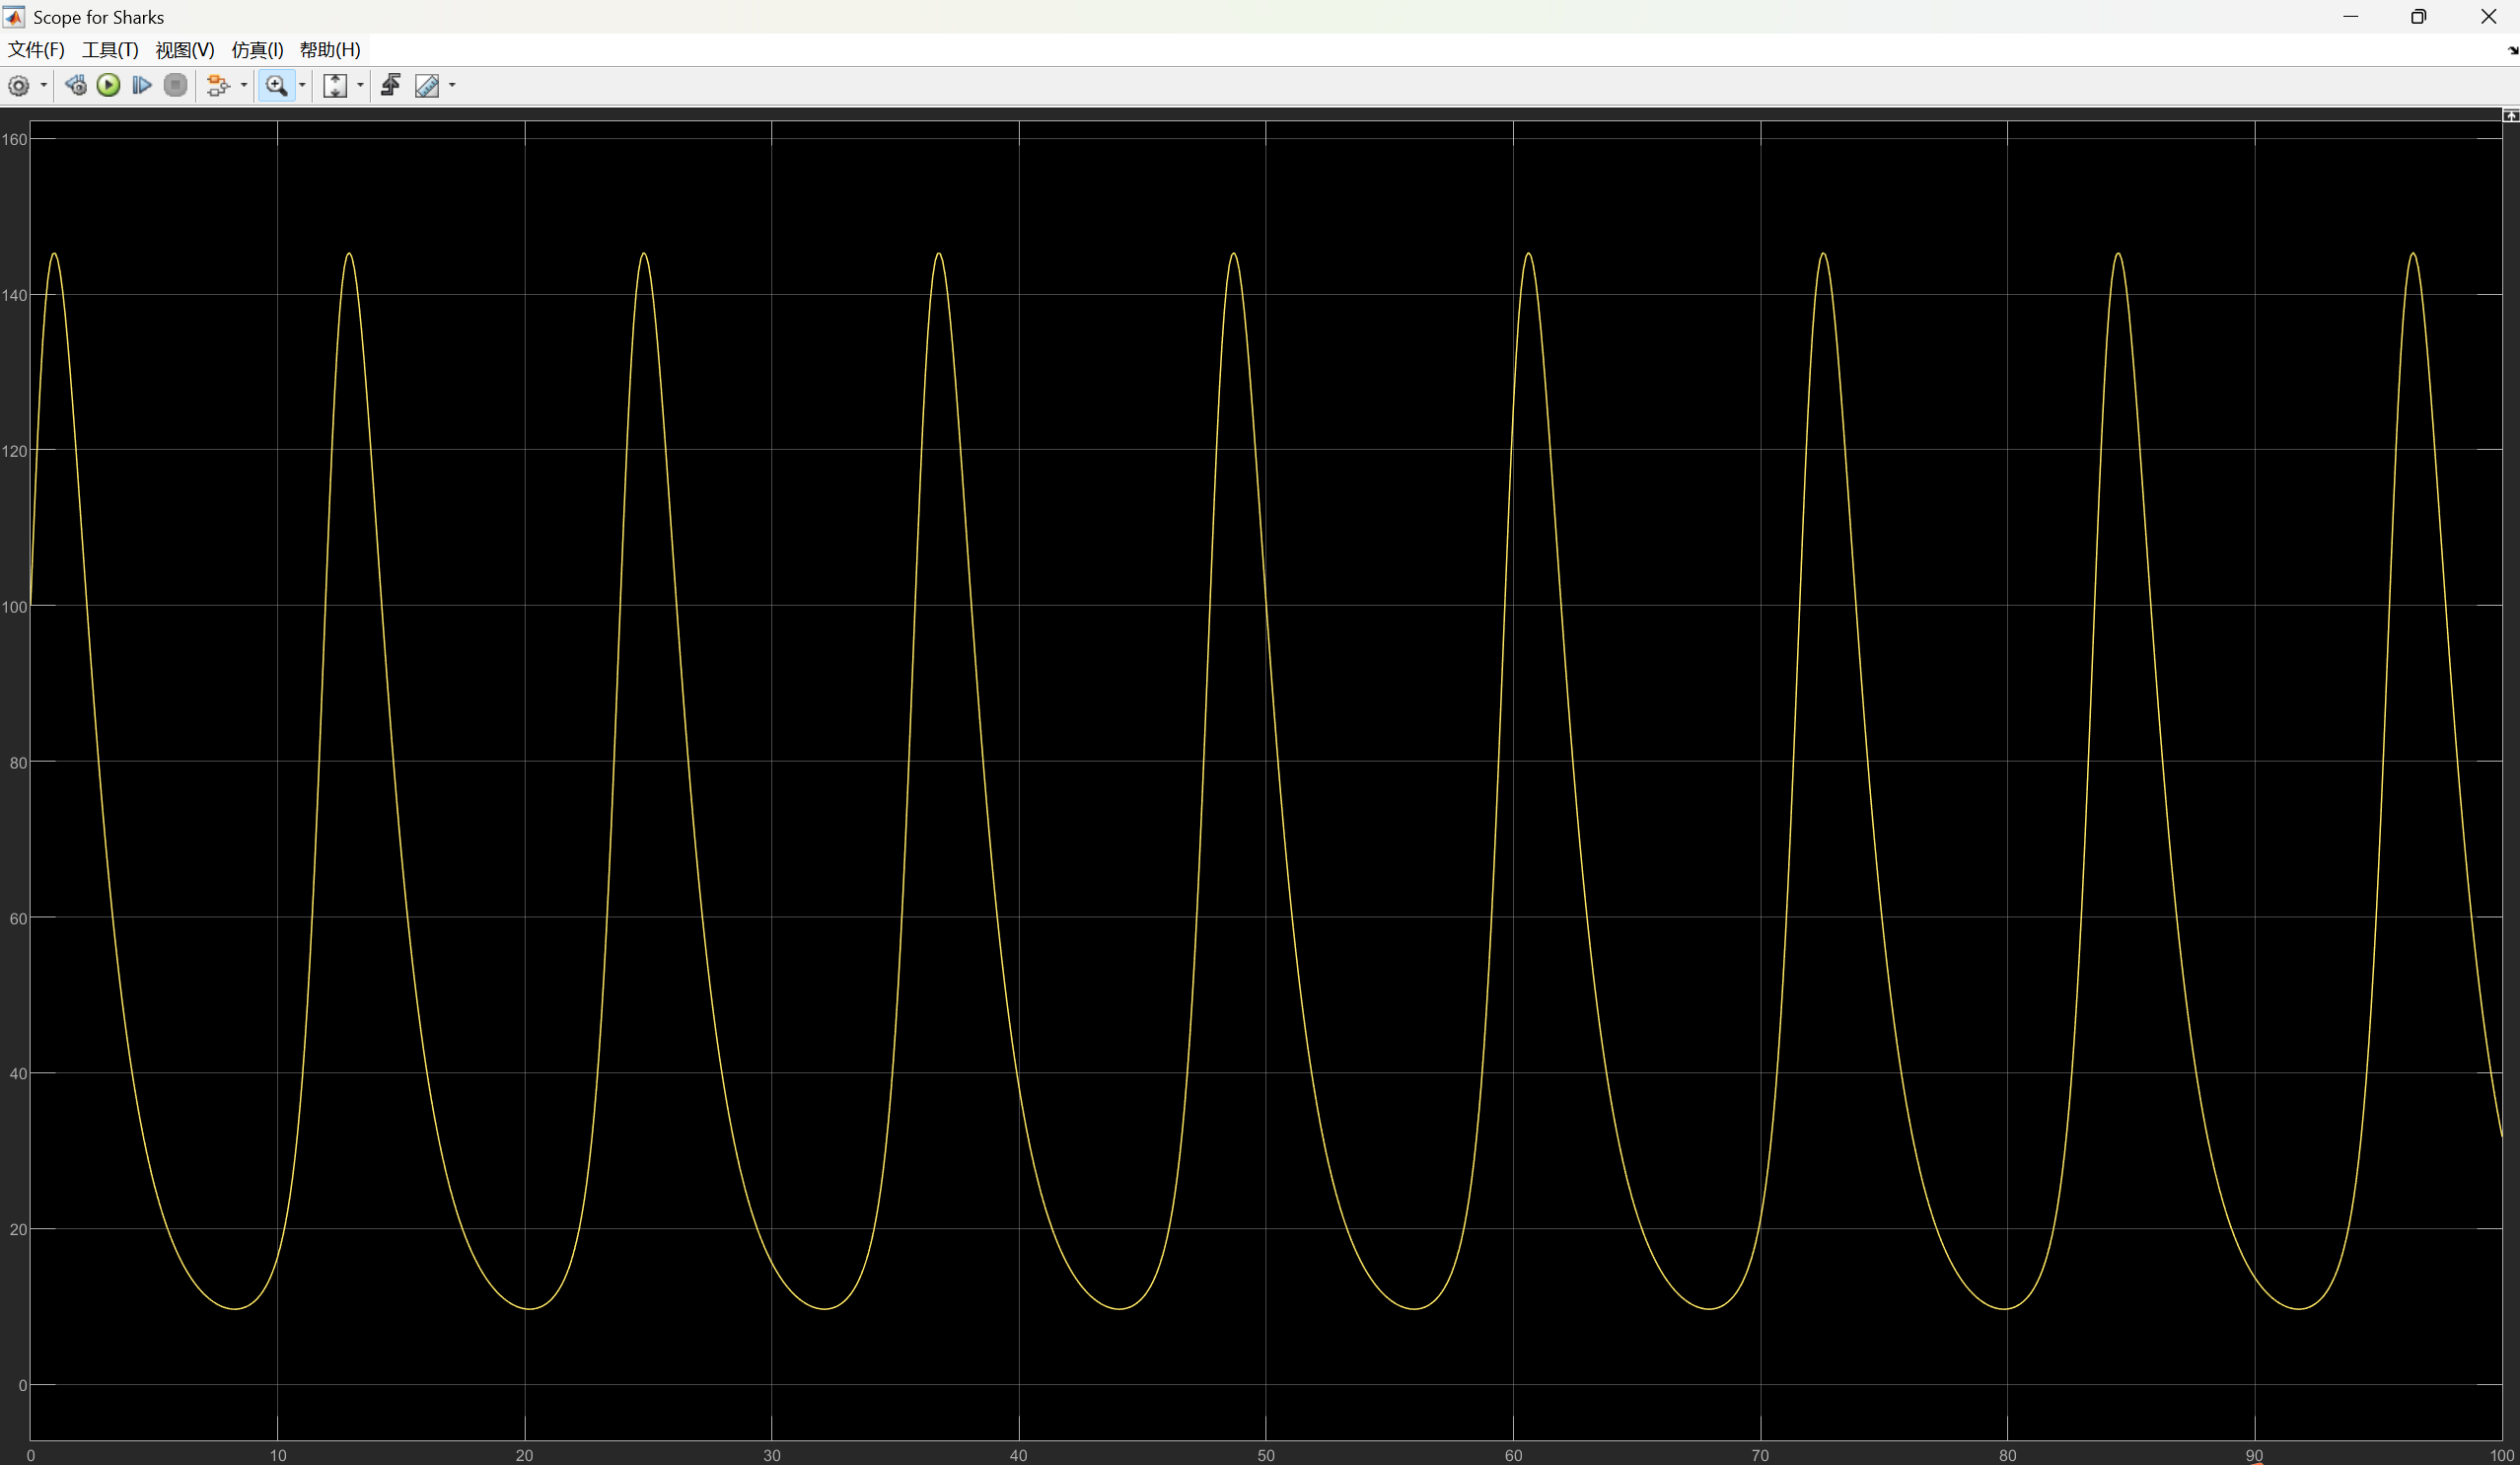
\includegraphics[width=\linewidth]{figure/HW1/ode4S0.1.png}
    \end{minipage}
    \hfill
    \begin{minipage}{0.48\textwidth}
        \centering
        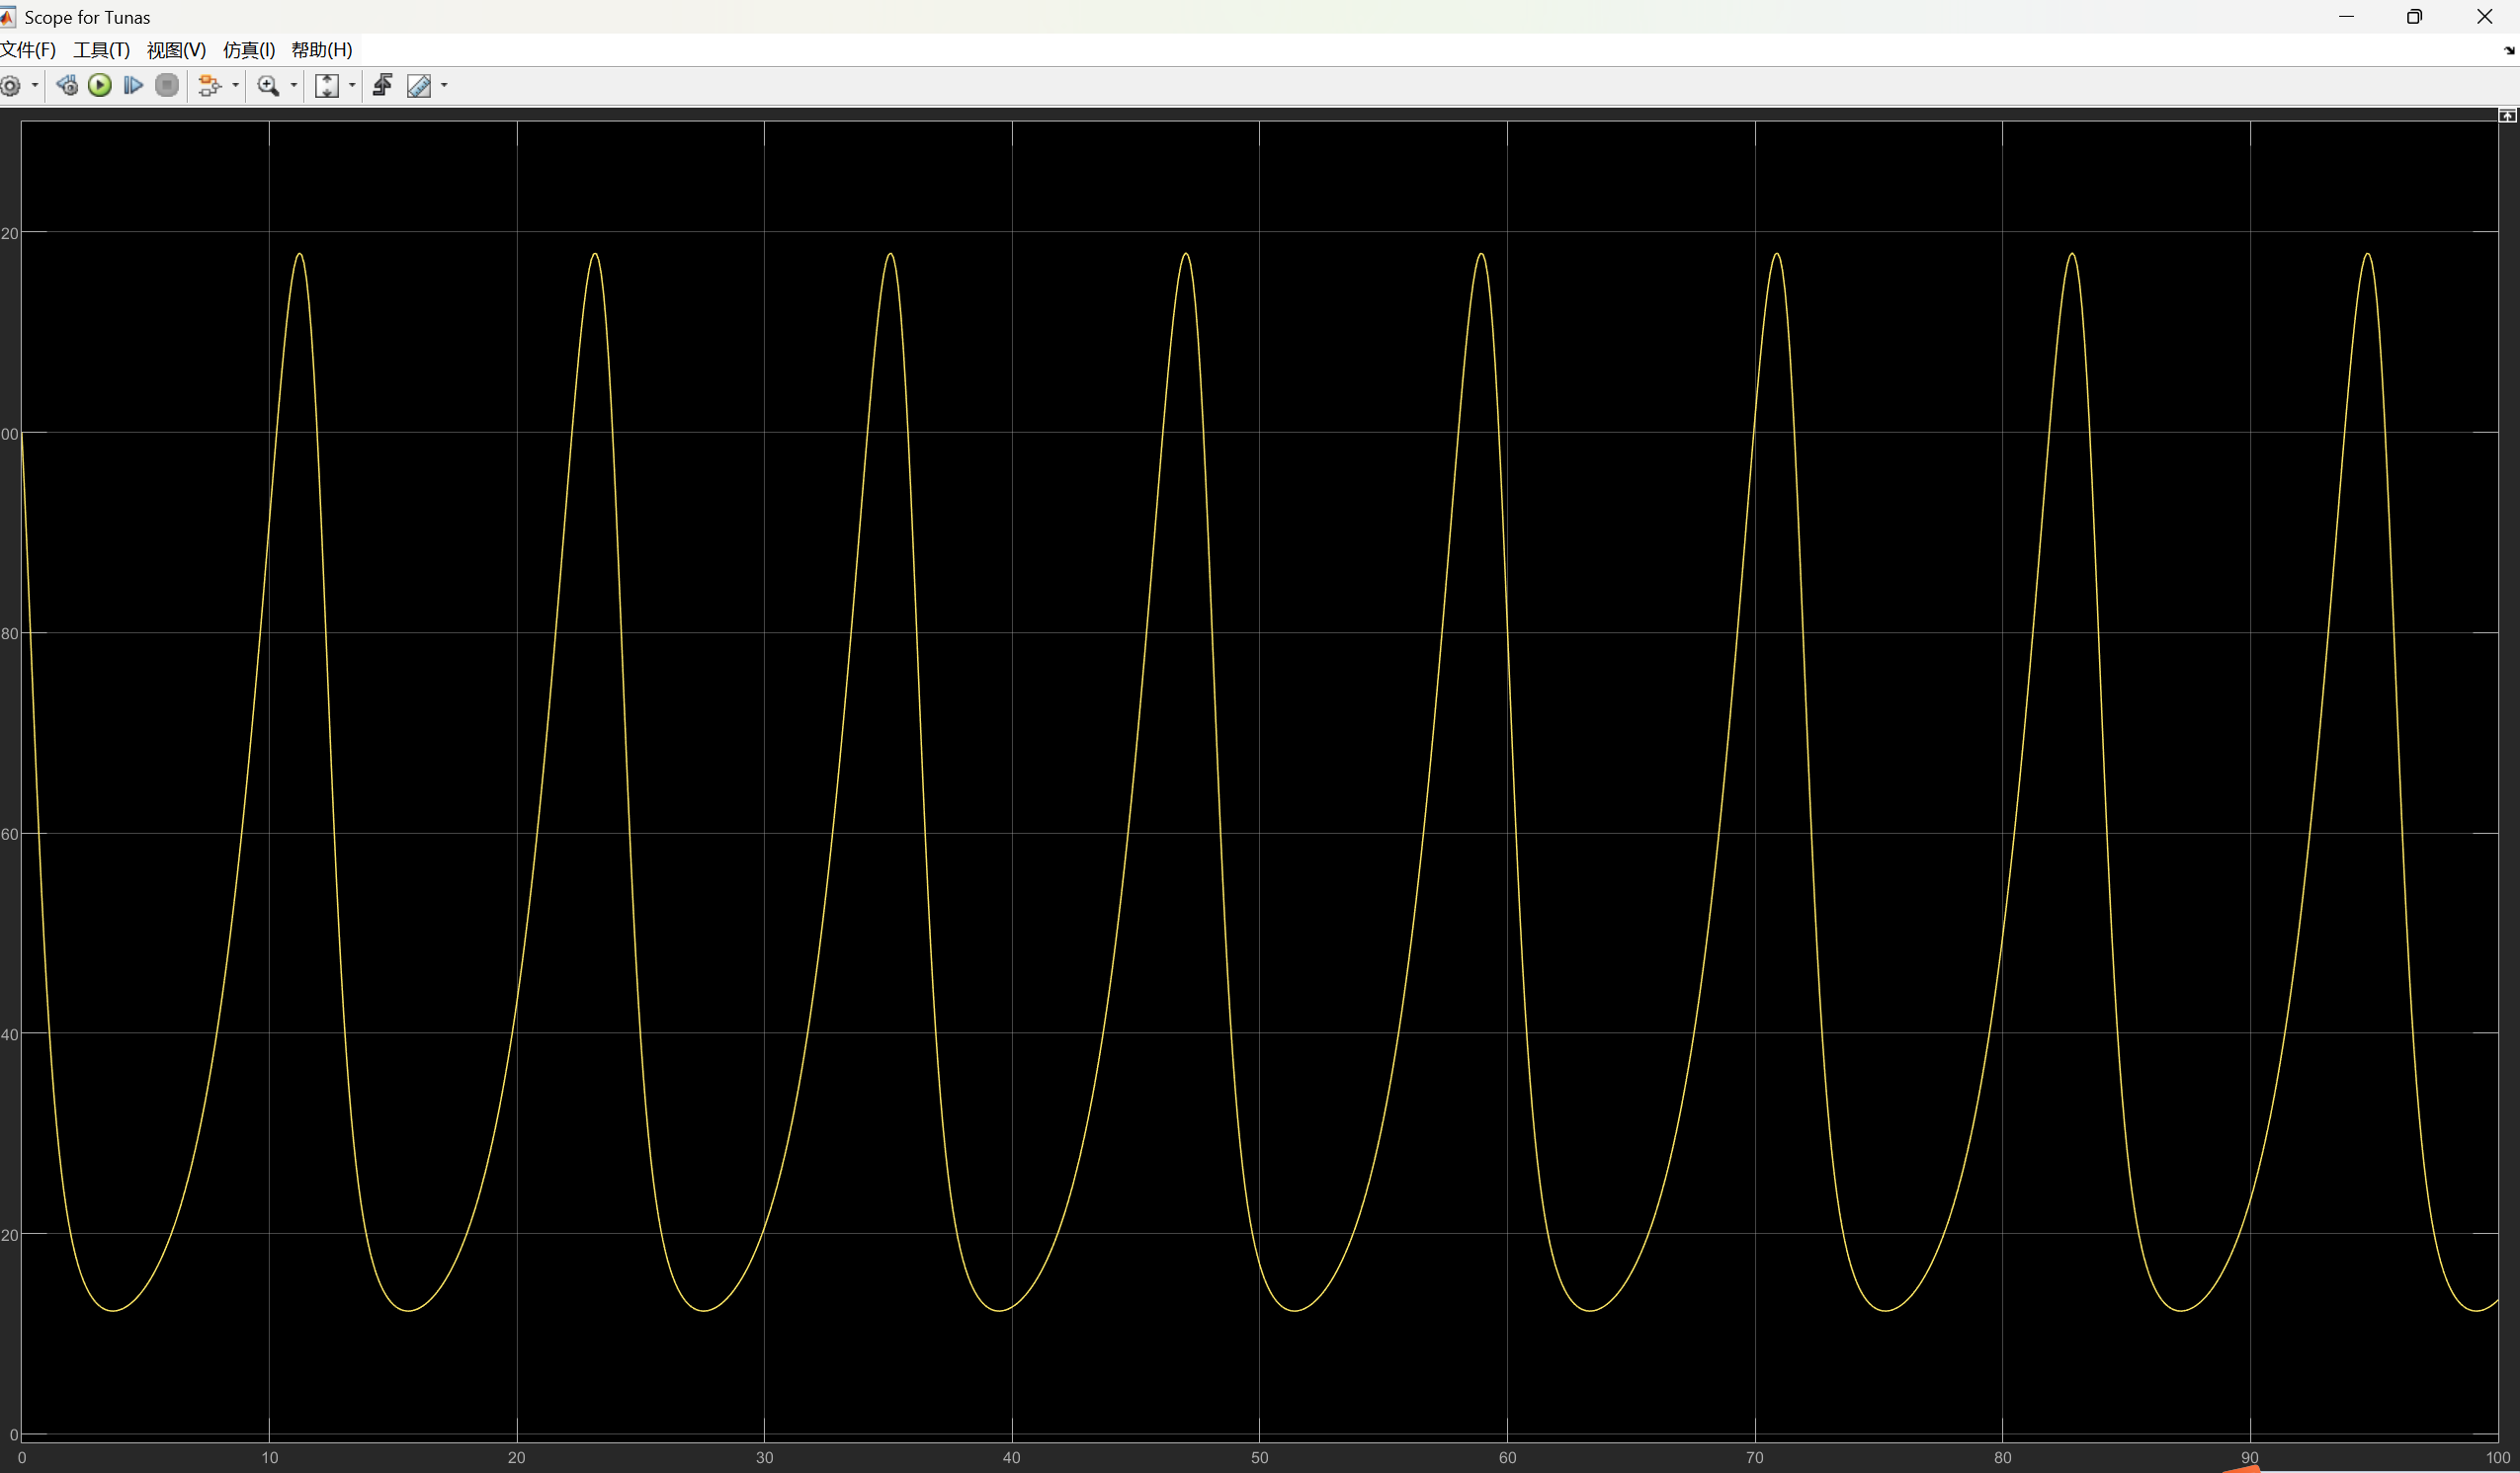
\includegraphics[width=\linewidth]{figure/HW1/ode4T0.1.png}
    \end{minipage}
    \caption{$\Delta t=0.1$ 时 ode4S 与 ode4T 数值结果}
\end{figure}
\par
四阶Runge-Kutta法在步长分别取 $\Delta t = 0.001$ 和 $\Delta t = 0.1$的情况下，结果并没有什么差异性。这与我们前文编程计算的结果相符。
\par
接下来考虑Euler法情况。
\begin{figure}[h]
    \centering
    \begin{minipage}{0.48\textwidth}
        \centering
        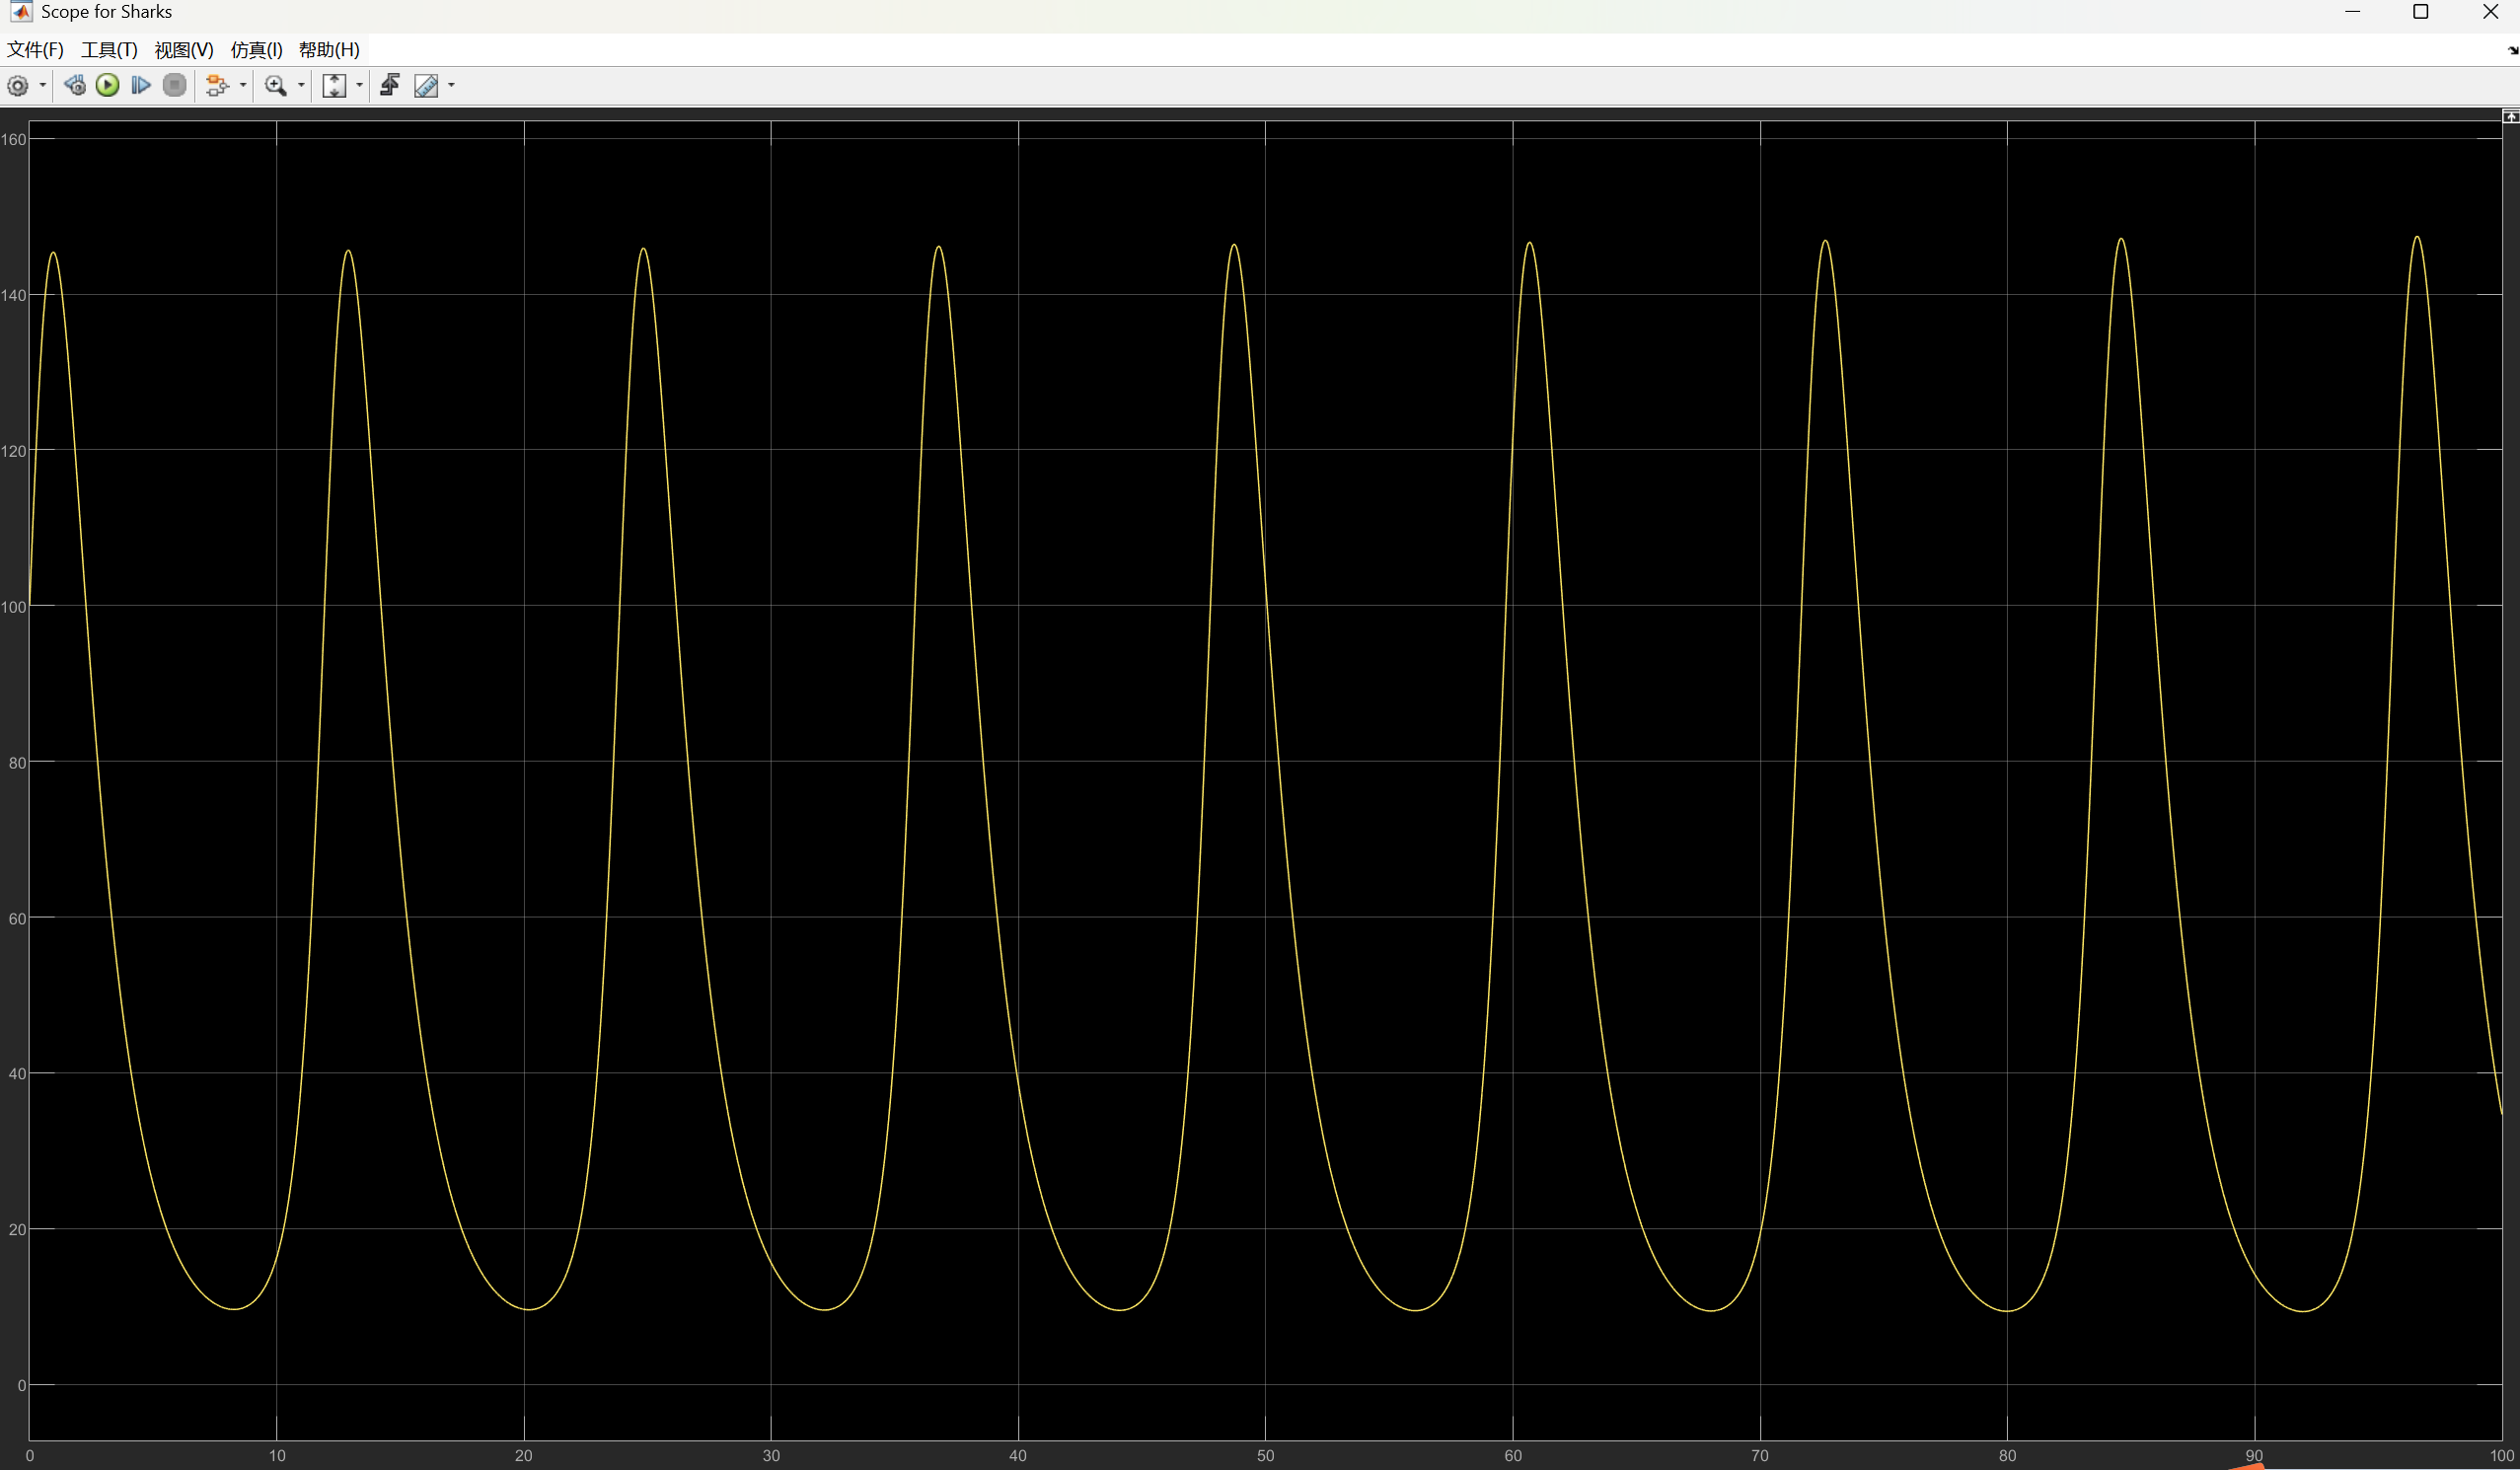
\includegraphics[width=\linewidth]{figure/HW1/ode1S0.001.png}
    \end{minipage}
    \hfill
    \begin{minipage}{0.48\textwidth}
        \centering
        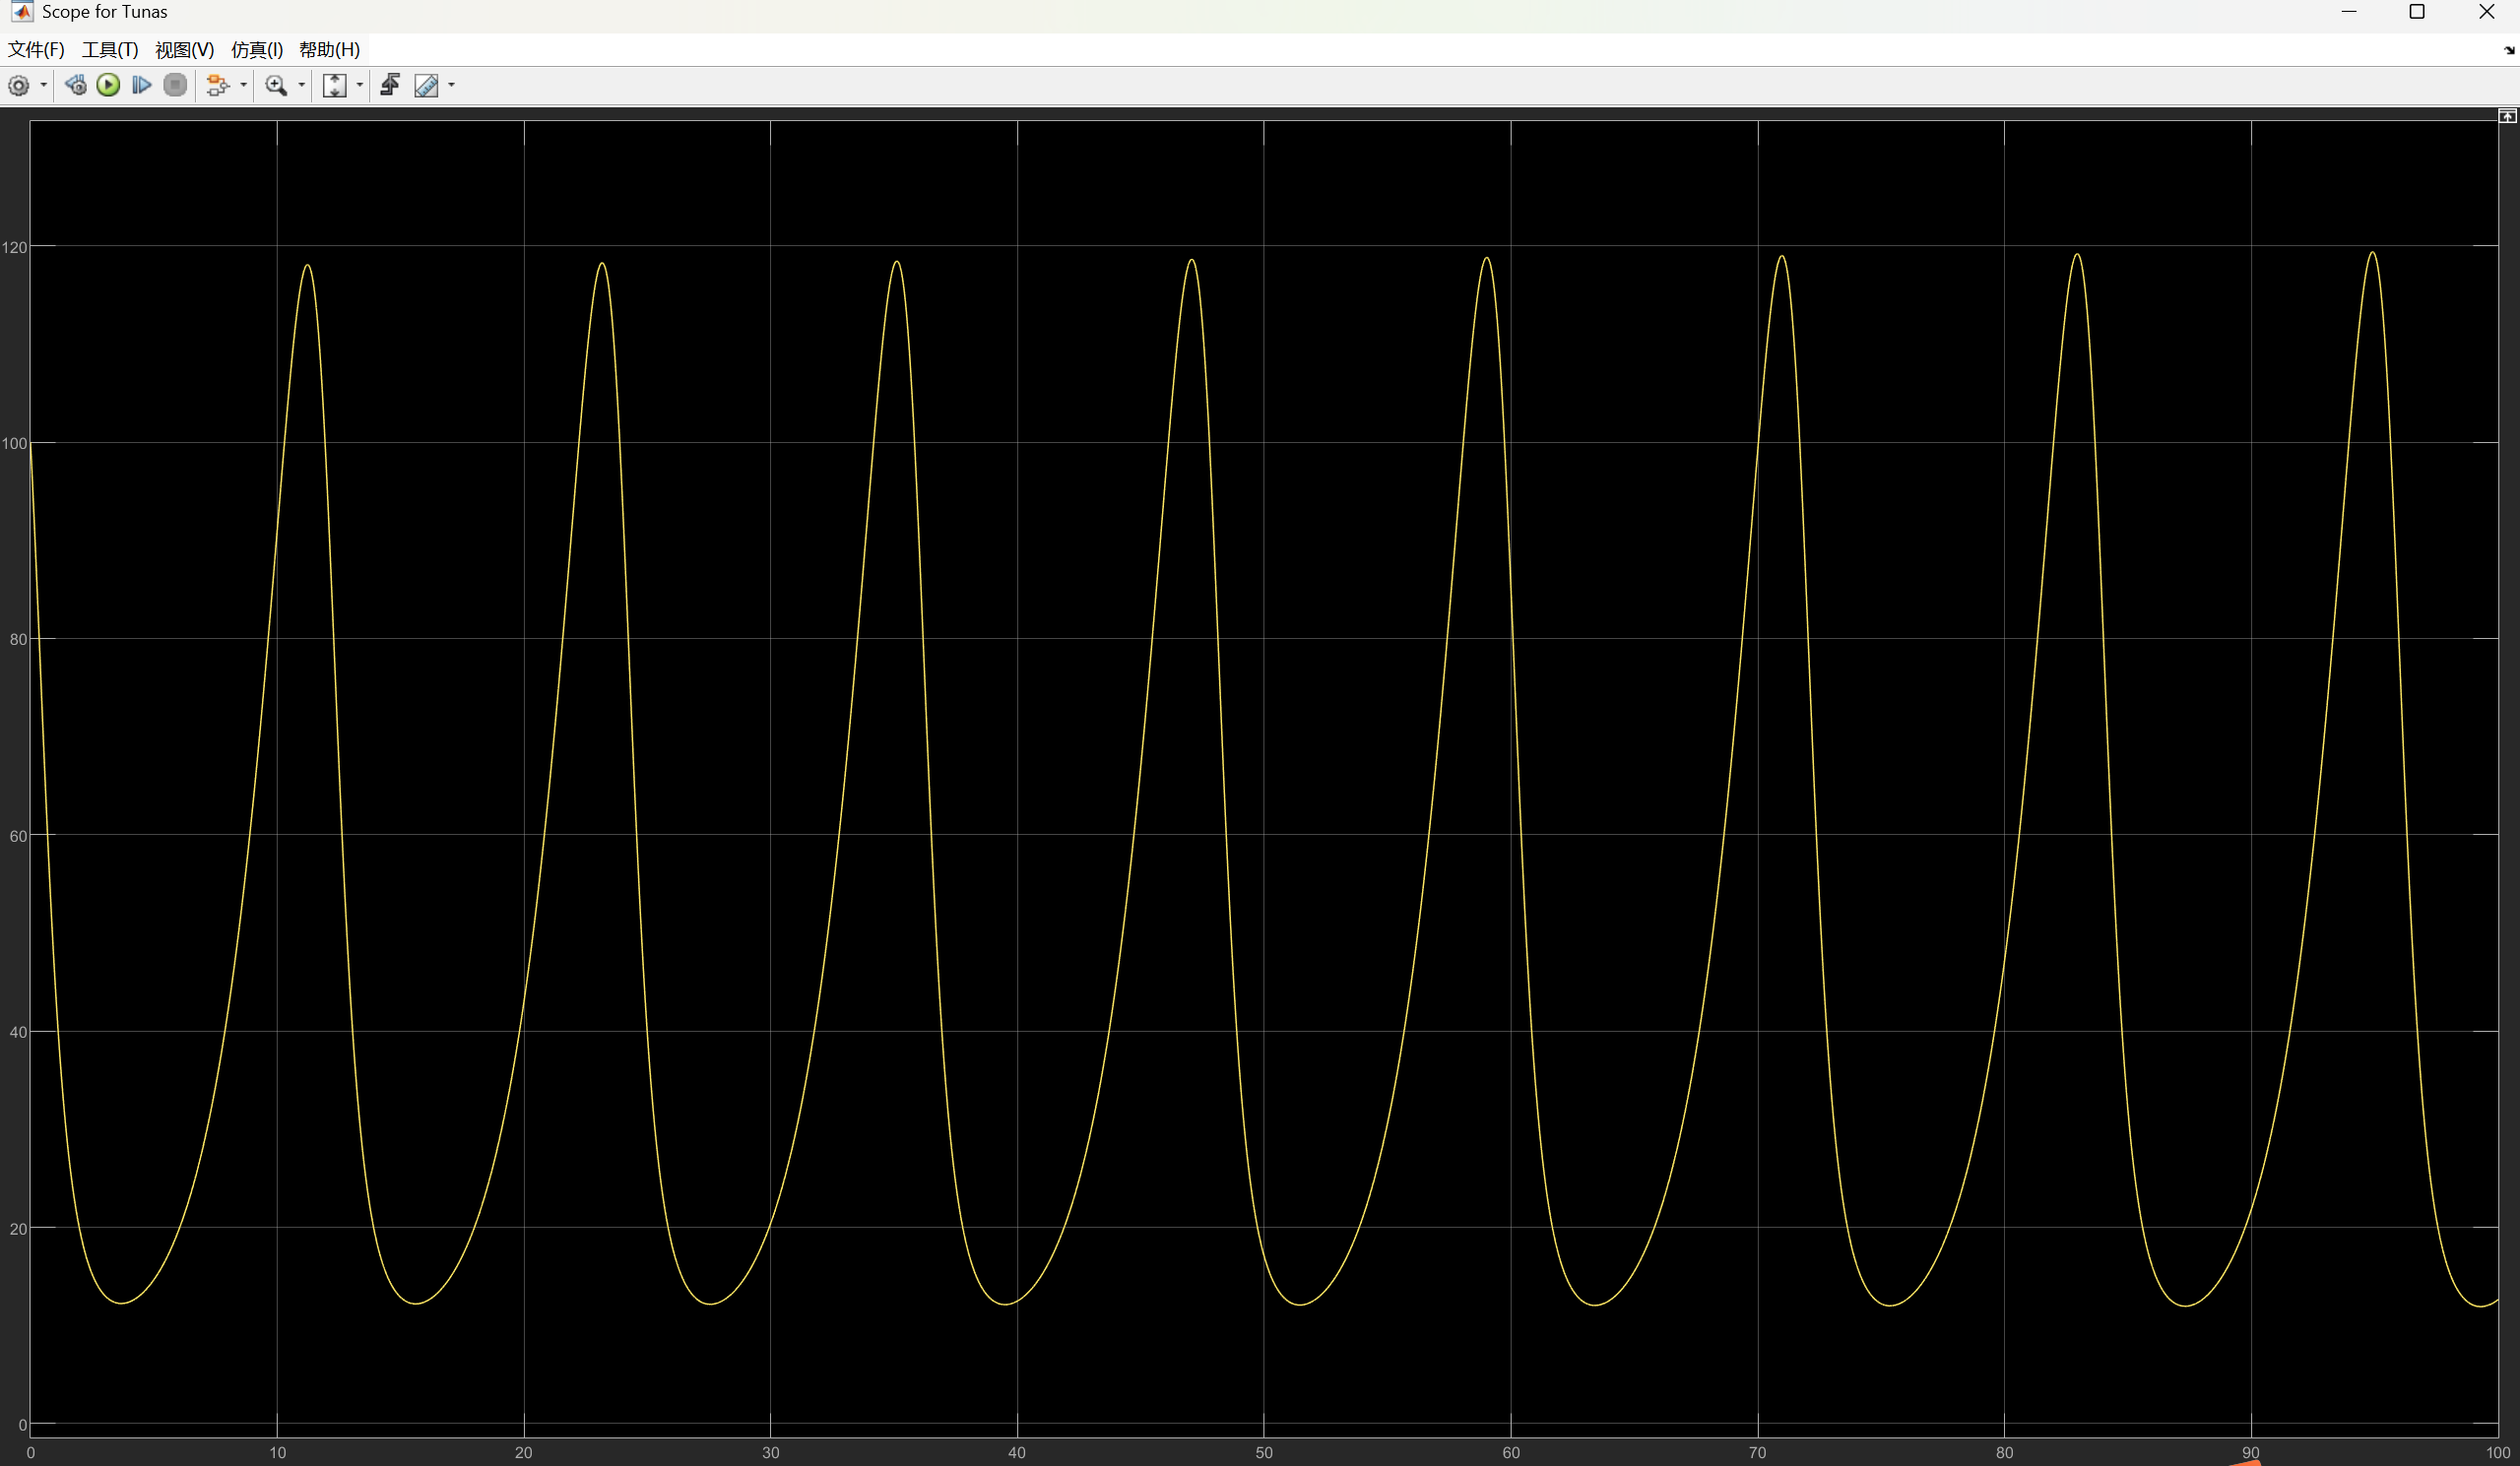
\includegraphics[width=\linewidth]{figure/HW1/ode1T0.001.png}
    \end{minipage}
    \caption{$\Delta t=0.001$ 时 ode1S 与 ode1T 数值结果}
\end{figure}
\begin{figure}[h]
    \centering
    \begin{minipage}{0.48\textwidth}
        \centering
        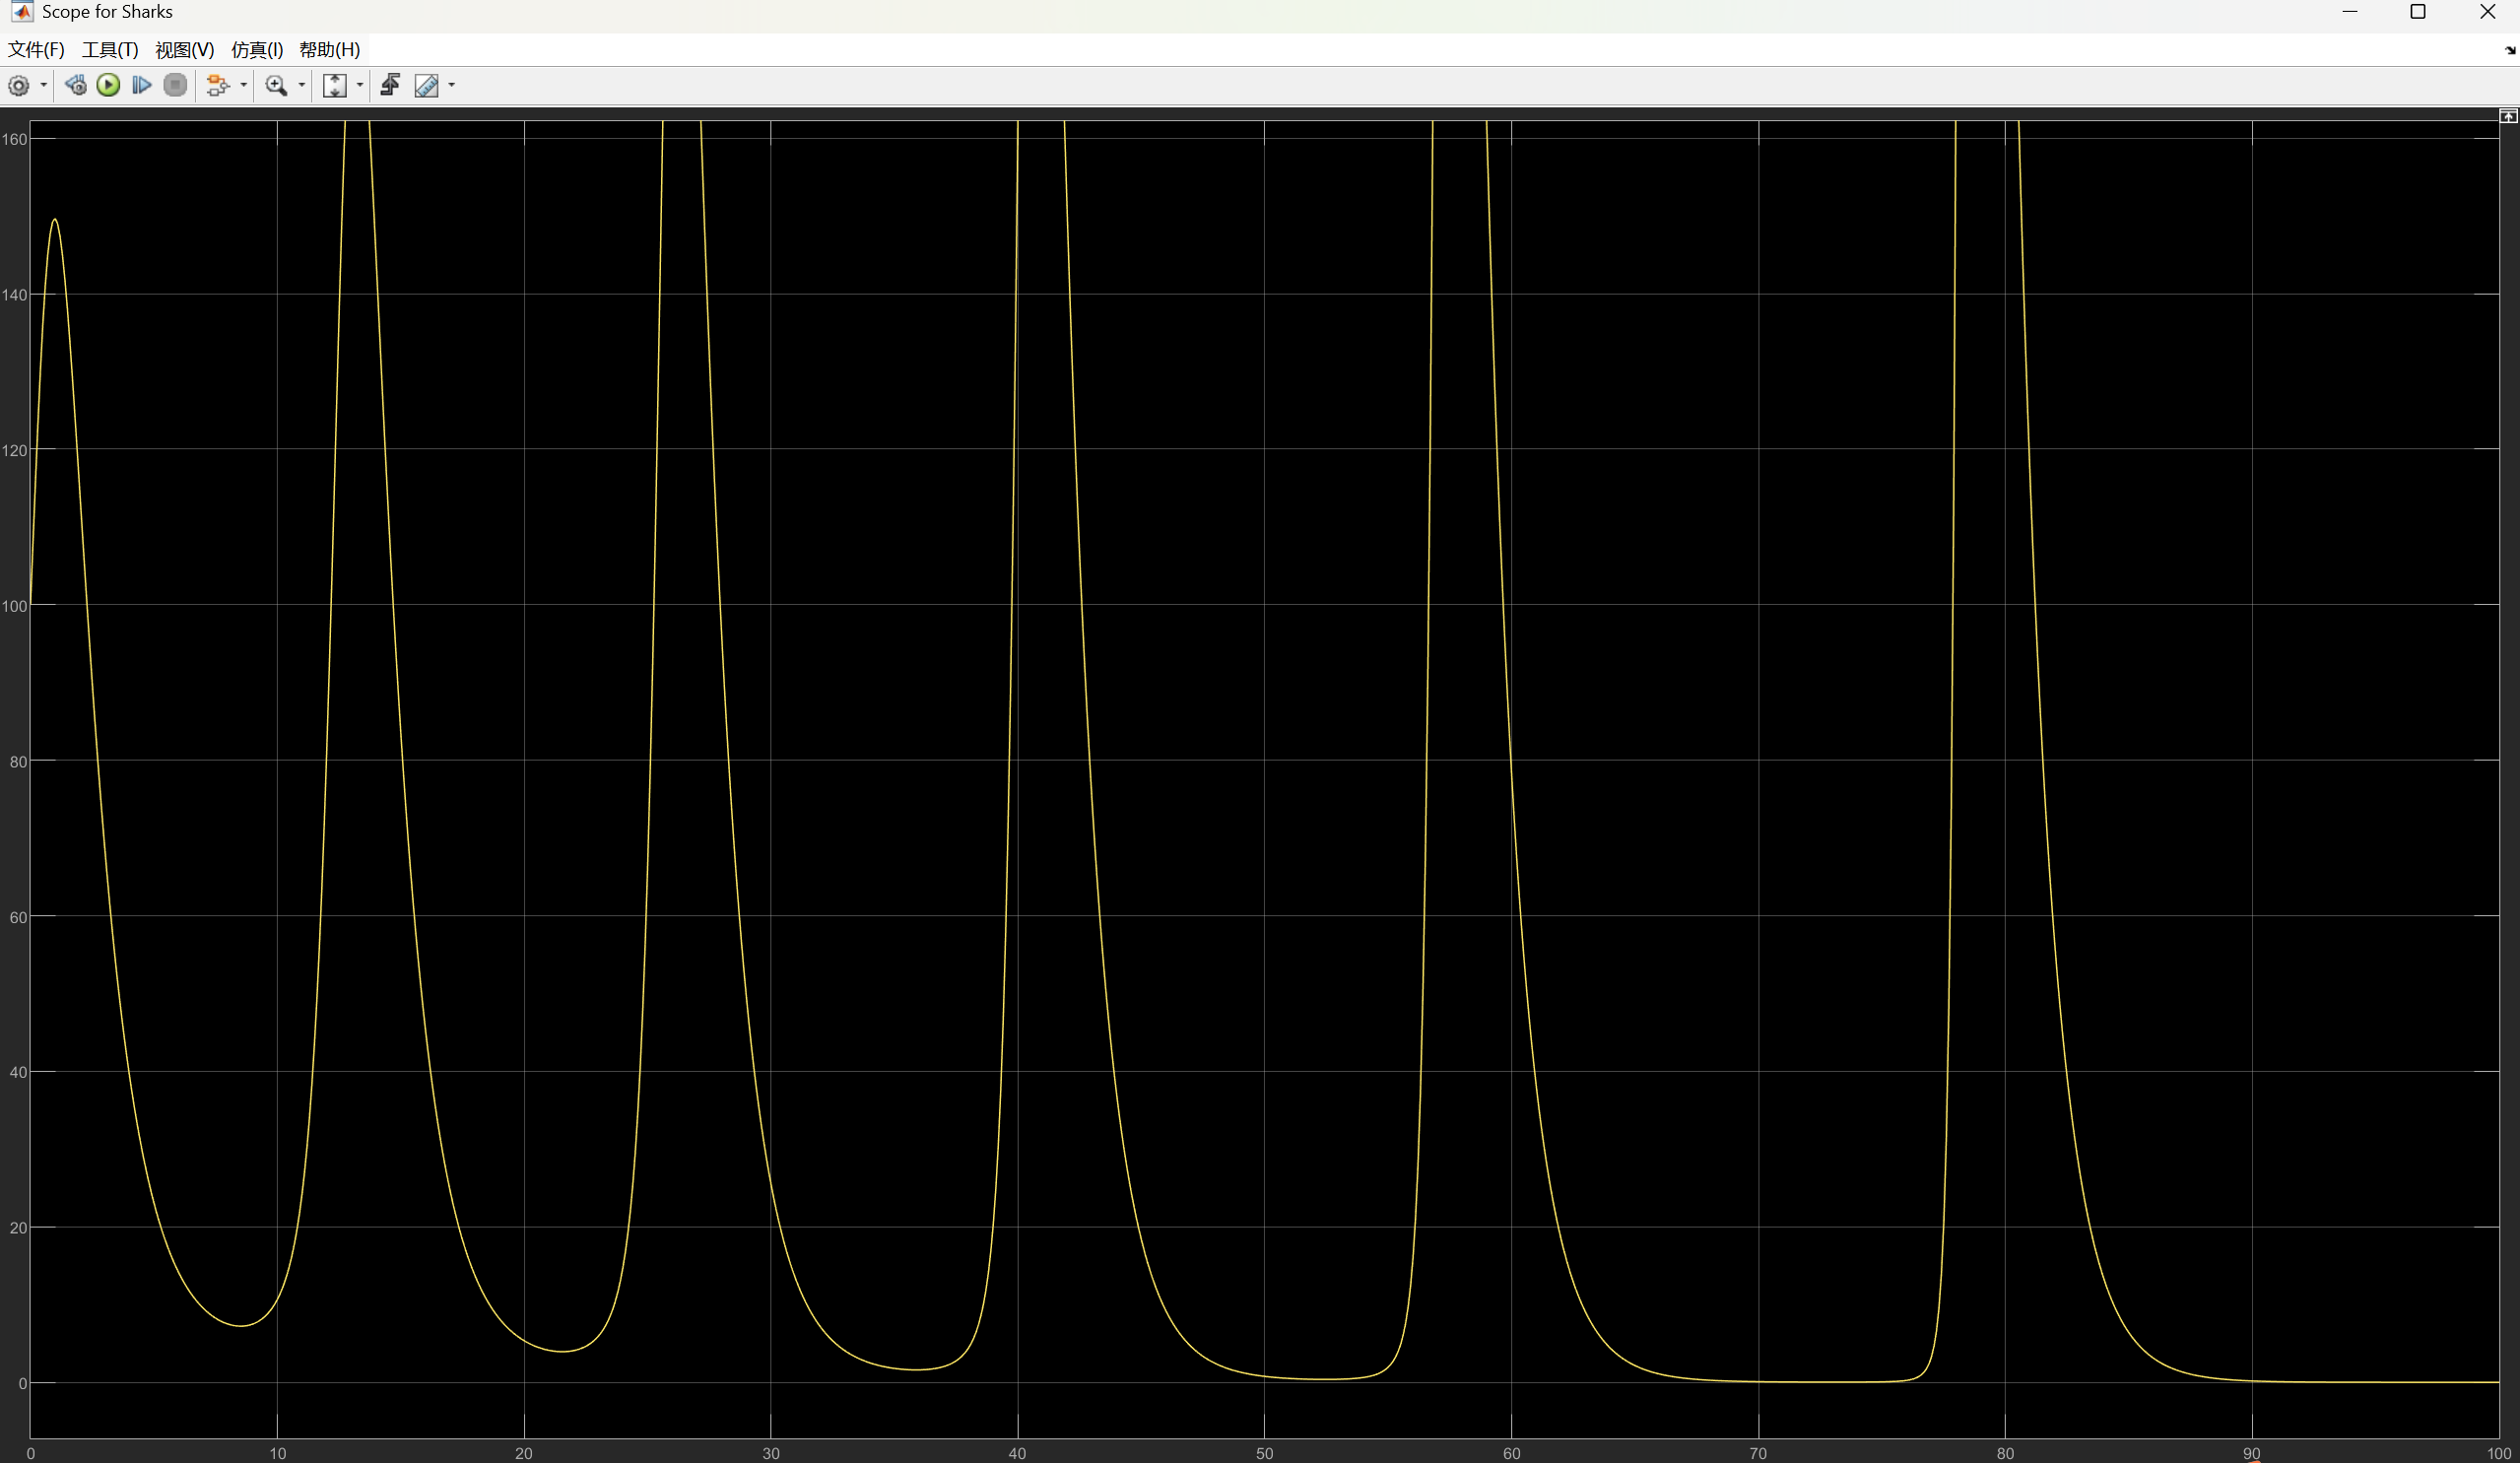
\includegraphics[width=\linewidth]{figure/HW1/ode1S0.1.png}
    \end{minipage}
    \hfill
    \begin{minipage}{0.48\textwidth}
        \centering
        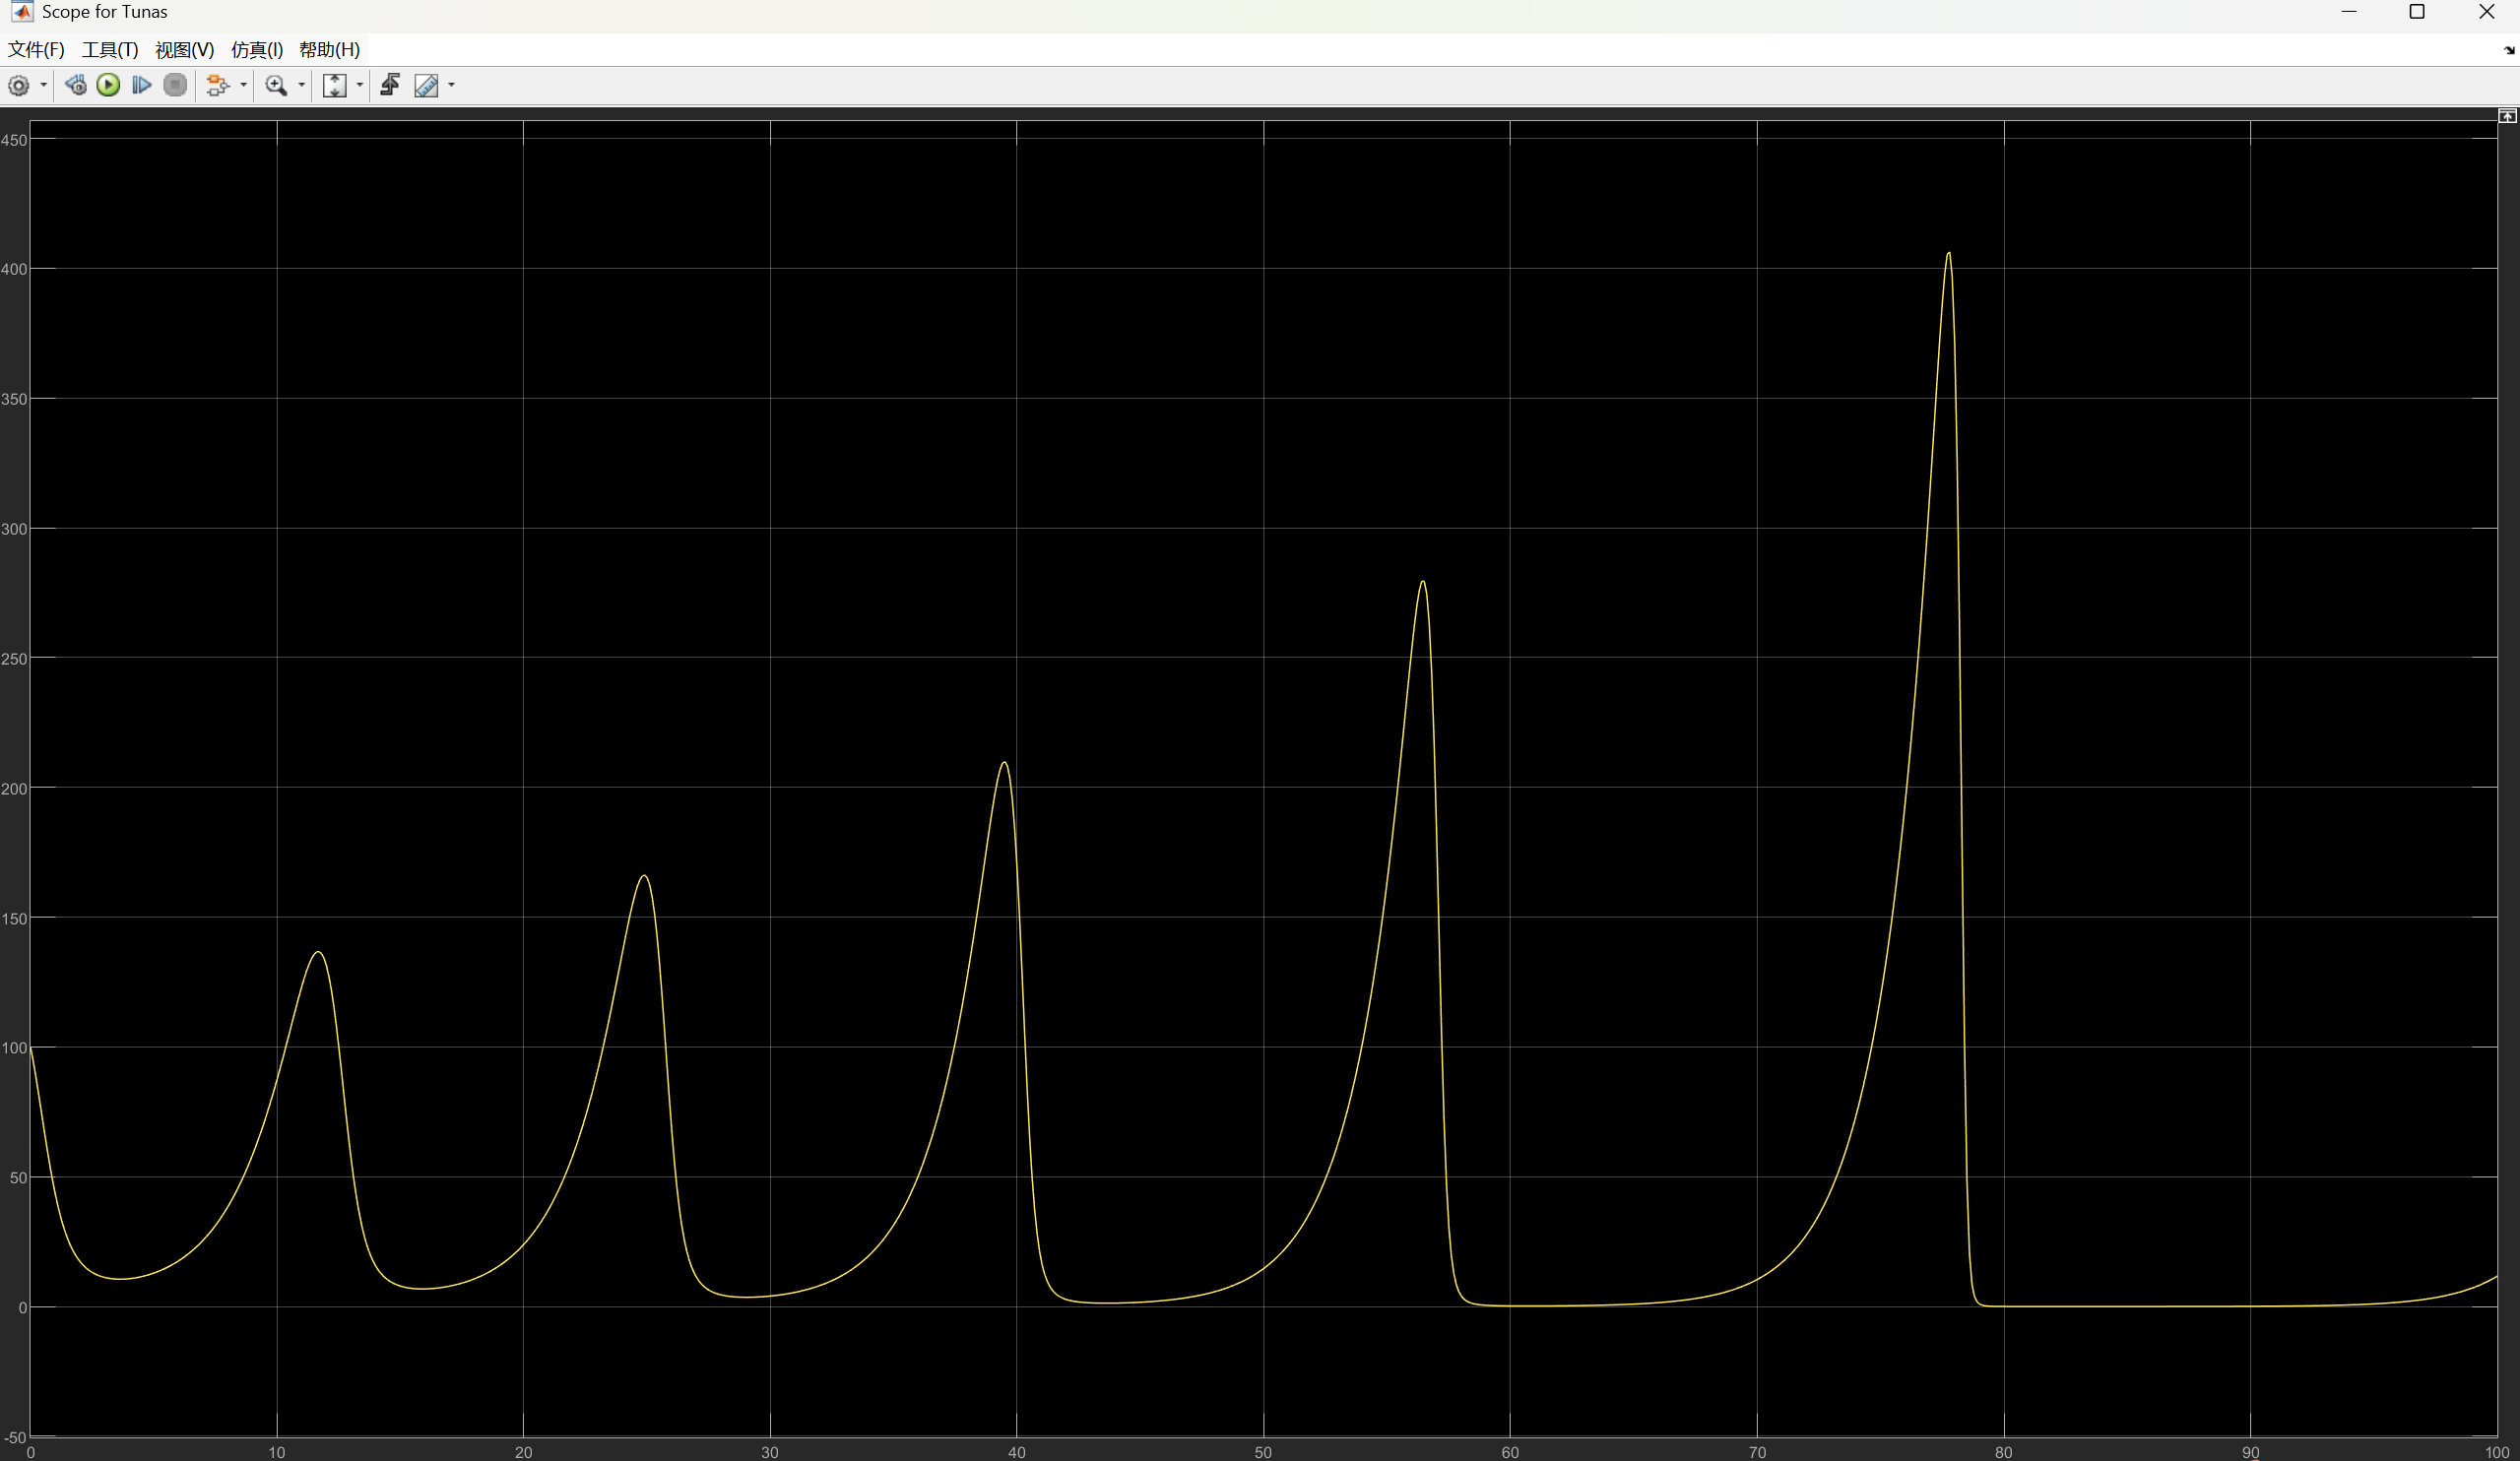
\includegraphics[width=\linewidth]{figure/HW1/ode1T0.1.png}
    \end{minipage}
    \caption{$\Delta t=0.1$ 时 ode1S 与 ode1T 数值结果}
\end{figure}
\par
不难注意到，这里Euler法在两种不同步长下仿真结果出现了显著差异。这与我们前文编程计算的结果相符，说明了显式Euler法的稳定性对步长敏感的特点。



\section{结果讨论}

数值实验表明：
\begin{itemize}
    \item 对于该非线性系统，显式Euler法的稳定性对步长敏感，步长需足够小（如0.001）才能保证稳定；
    \item RK4法稳定性远优于Euler法，即使步长增大至0.1仍能获得可靠结果；
    \item 实际计算中，推荐使用高阶方法（如RK4）以兼顾精度与效率。
\end{itemize}

本道题目的用意在于让我们初步了解利用MATLAB进行仿真的方法。对于题目反映的生态学等方面的内涵，我们在此不做讨论。



\section{代码附录}
\inputMATLAB{codes/HW1/main.m}
\inputMATLAB{codes/HW1/EulerMethod.m}
\inputMATLAB{codes/HW1/ode45Solver.m}
\inputMATLAB{codes/HW1/rk4Method.m}
